\documentclass[11pt,a4paper]{article}

\usepackage[utf8]{inputenc}
\usepackage[T1]{fontenc}
\usepackage{lmodern}
\usepackage[margin=1.85cm]{geometry}
\usepackage{amsmath}
\usepackage{booktabs}
\usepackage{array}
\usepackage{tabularx}
\usepackage{longtable}
\usepackage{graphicx}
\usepackage{xcolor}
\usepackage{hyperref}
\usepackage{microtype}
\usepackage{caption}
\usepackage{float}
\usepackage{fancyhdr}
\usepackage{enumitem}

\definecolor{navy}{HTML}{102A43}
\definecolor{blue}{HTML}{1677B8}
\definecolor{green}{HTML}{2A9D6F}
\definecolor{light}{HTML}{F4F7FA}
\definecolor{muted}{HTML}{627D98}
\hypersetup{colorlinks=true,linkcolor=blue,urlcolor=blue,
pdftitle={Nationwide France Apartment Valuation: Phase 4 Benchmark},pdfauthor={Badr Ettousy}}
\graphicspath{{../../visuals/phase4/}}
\captionsetup{font=small,labelfont=bf}
\setlength{\parskip}{0.38em}
\setlength{\parindent}{0pt}
\renewcommand{\arraystretch}{1.15}
\pagestyle{fancy}
\fancyhf{}
\fancyhead[L]{\small\textcolor{muted}{France AVM --- Phase 4 national benchmark}}
\fancyhead[R]{\small\textcolor{muted}{Badr Ettousy}}
\fancyfoot[C]{\thepage}
\setlength{\headheight}{14pt}

\newenvironment{statusbox}{\begin{center}\begin{minipage}{0.92\textwidth}\textcolor{navy}{\rule{\textwidth}{0.8pt}}\vspace{0.5em}}{\vspace{0.5em}\textcolor{navy}{\rule{\textwidth}{0.8pt}}\end{minipage}\end{center}}
\newcommand{\metriccard}[2]{\colorbox{light}{\begin{minipage}[c][1.45cm][c]{0.215\textwidth}\centering\textcolor{navy}{\Large\textbf{#1}}\\[-0.1em]\small\textcolor{muted}{#2}\end{minipage}}}

\title{\textcolor{navy}{\textbf{Nationwide France Apartment Valuation}}\\[0.25em]
\large Phase 4 Data Engineering, Leakage Controls and\\Chronological Model Benchmark}
\author{Badr Ettousy}
\date{27 August 2026\\\small Empirical benchmark edition}

\begin{document}
\maketitle

\begin{abstract}
This report evaluates one region-aware CatBoost automated valuation model
on 350,399 untouched 2025 apartment sales represented in nationwide Geo-DVF.
Development uses 2021--2023 and model selection uses 2024. The selected model reaches EUR
41,936 MAE, 13.50\% median absolute
percentage error and $R^2=0.8490$. It improves MAE by EUR
10,957 relative to a training-only hierarchical
geographic median baseline. All comparable-sale features enforce a minimum 90-day information lag.
\end{abstract}

\textbf{Keywords:} automated valuation model; Geo-DVF; France; CatBoost;
historical comparable sales; chronological validation; regional robustness.

\tableofcontents
\clearpage

\section{Executive assessment}

Phase 4 extends the earlier Paris research into one national apartment model. The
central design choice is comparability rather than superficial feature parity:
Paris-only transport, school, park, noise and building snapshots are not copied
into other regions without a nationally uniform source contract. The national
model instead uses DVF property attributes, transaction time, hierarchical
territorial identity, global geometry and point-in-time comparable-sale evidence.


\begin{center}
\metriccard{EUR 41,936}{2025 model MAE} \hfill
\metriccard{13.50\%}{2025 median APE} \hfill
\metriccard{66.97\%}{within $\pm 20\%$} \hfill
\metriccard{90.28\%}{90\% interval coverage}
\end{center}


\subsection*{Decision status}
\begin{itemize}[leftmargin=1.5em]
\item The data, benchmark and reporting protocols are fully specified and tested.
\item The frozen 2025 result covers 350,399 transactions; no 2025 outcome influenced model selection.
\item Regional MAE is interpreted beside MdAPE, hit rate and test-row count.
\item The output is an automated indication, not a certified appraisal.
\end{itemize}

\section{Research objective and contributions}

The target is total transaction value in euros for an ordinary apartment sale.
The study asks whether one model can learn heterogeneous French markets while
preserving local evidence and honest temporal evaluation. Its contributions are:
\begin{enumerate}[leftmargin=1.6em]
\item chunk-safe processing of the national annual Geo-DVF archives;
\item explicit support for Corsican and overseas territorial identifiers;
\item spherical H3 and Cartesian location features valid outside Lambert-93;
\item local comparables subject to a 90-day information-availability lag;
\item a training-only hierarchical postcode-to-national median baseline;
\item a 2021--2023/2024/2025 chronological benchmark with paired bootstrap uncertainty;
\item region and sufficiently sized department diagnostics;
\item atomic artifacts, checksums, a reusable production bundle and inference CLI.
\end{enumerate}


\begin{figure}[H]
\centering
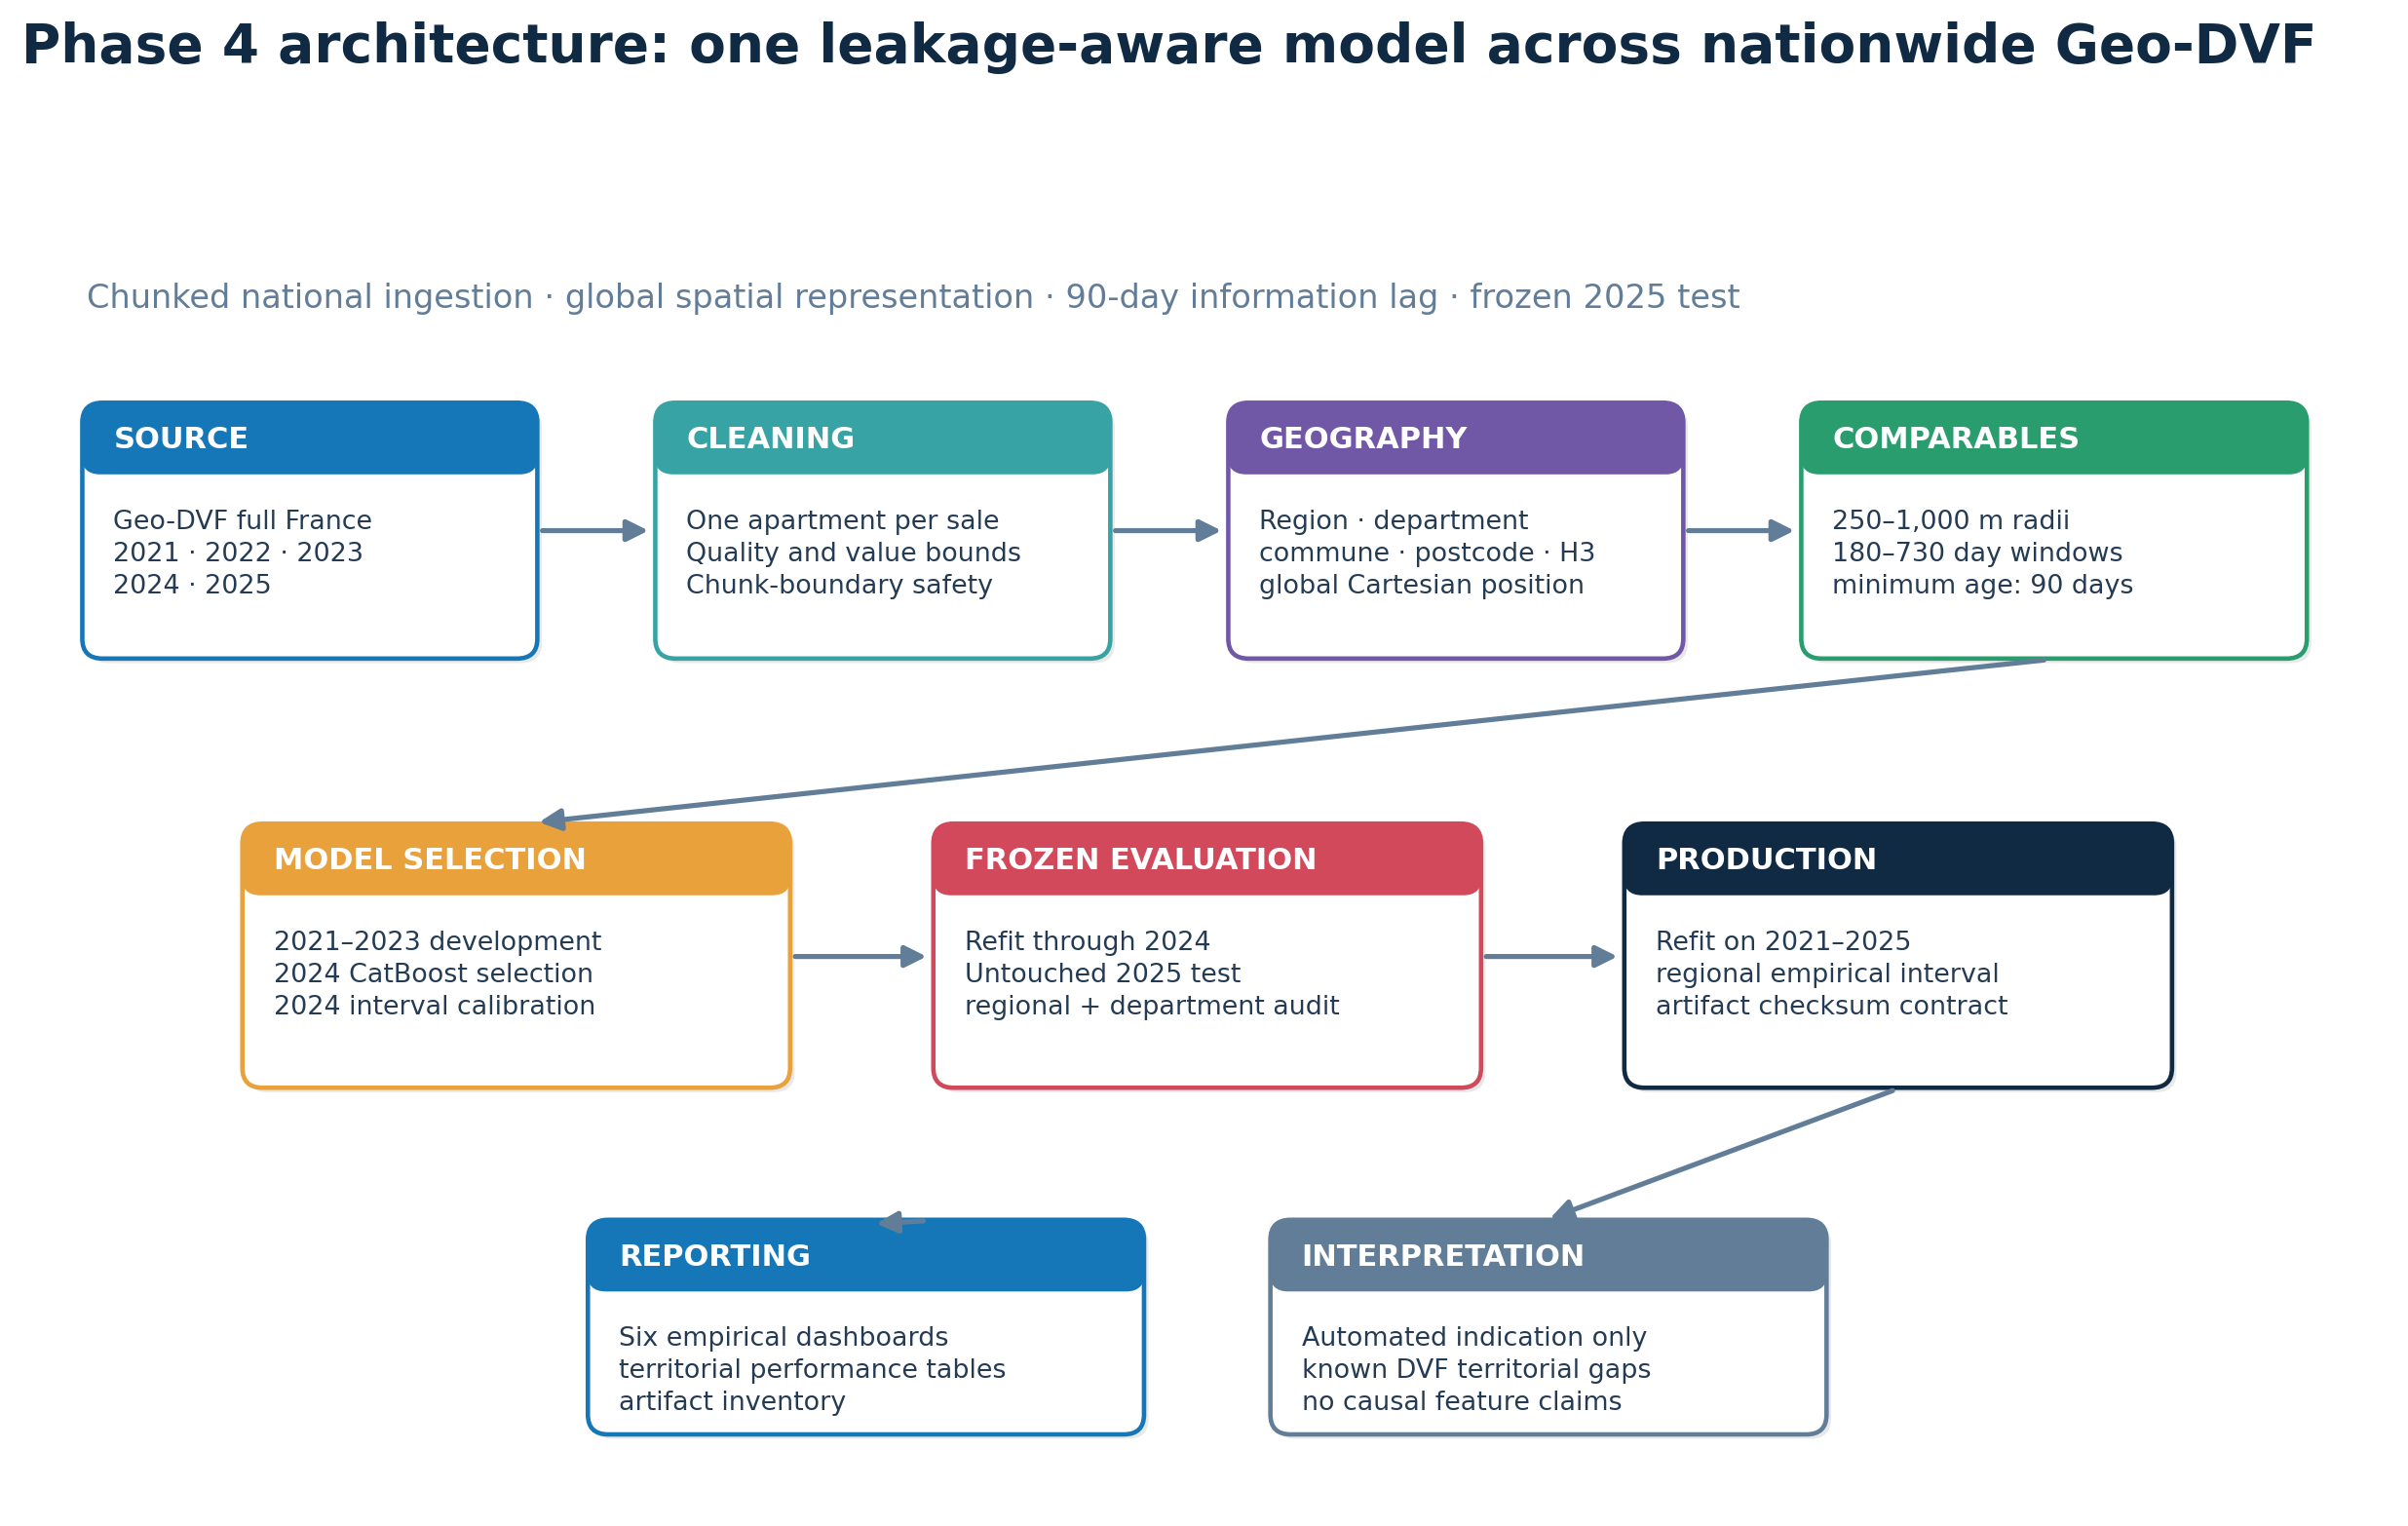
\includegraphics[width=\textwidth]{phase4_national_pipeline.png}
\caption{Phase 4 source-to-report architecture and chronological evaluation design.}
\label{fig:architecture}
\end{figure}


\section{Data source and analytical cohort}

The source is the normalized and geolocated Geo-DVF annual full archive for
2021--2025. CSV files are streamed in bounded chunks. The last mutation in each
chunk is carried into the next chunk so a multi-line transaction is never
classified before all its property rows are available.

The cohort retains \emph{Vente} mutations containing exactly one apartment and
no house or commercial premises. Dependencies such as a cellar or parking place
may remain bundled in the mutation consideration. Required fields are date,
transaction value, apartment surface, commune and valid WGS84 coordinates.
Broad national quality bounds are 9--300 m$^2$, EUR 10,000--10,000,000 and EUR
100--30,000 per m$^2$.

The audited Gold table contains 1,850,486 sales from
2021-01-01 through 2025-12-31, representing
97 departments and 17 regions.

Geo-DVF contains no open observations for departments 57, 67, 68, 976.
``Nationwide'' therefore means every territory represented upstream, not every
French department without exception.

\section{Feature engineering contract}

The fitted contract contains 45 inputs:
38 numeric and
7 categorical variables. The current
transaction's target and price per square metre are excluded.

\begin{table}[H]
\centering
\caption{Phase 4 feature families.}
\begin{tabularx}{\textwidth}{p{3.4cm}rX}
\toprule
Family & Inputs & Role \\
\midrule
Property & 6 & Surface, rooms, address number, lots and scale/density transforms \\
Calendar & 4 & Seasonality and elapsed market time \\
Global location & 5 & WGS84 and unit-sphere Cartesian coordinates \\
Territorial identity & 7 & Region, department, commune, postcode and H3 r7/r8/r9 \\
Historical comparables & 23 & Lagged counts, medians, dispersion, similarity, age, distance and momentum \\
\bottomrule
\end{tabularx}
\end{table}

\subsection{Global spatial representation}

Lambert-93 is unsuitable for overseas departments. Longitude $\lambda$ and
latitude $\phi$ are therefore supplemented by unit-sphere coordinates
\begin{equation}
(x,y,z)=(\cos\phi\cos\lambda,\cos\phi\sin\lambda,\sin\phi),
\end{equation}
and H3 cells. Nearby transactions are queried using haversine distance within
each department.

\subsection{Leakage-safe comparable sales}

For target sale $i$ at date $t_i$, candidate $j$ is eligible only if
\begin{equation}
90 \le t_i-t_j \le 730\quad\text{days},\qquad d(i,j)\le1{,}000\text{ m}.
\end{equation}
Windows at 180, 365 and 730 days and radii at 250, 500 and 1,000 metres produce
counts and median prices per square metre. Exponential recency/distance weights,
surface and room similarity, effective sample size, dispersion and momentum
summarize local evidence. The current transaction cannot become its own input.

\begin{table}[H]
\centering
\caption{Primary leakage and integrity controls.}
\begin{tabularx}{\textwidth}{p{4.4cm}X}
\toprule
Risk & Enforced control \\
\midrule
Mutation target duplication & One row only after transaction-level local-type audit \\
Future comparable sales & Minimum 90-day age and positive chronological difference \\
Target-derived leakage & Current value and price/m$^2$ excluded from fitted inputs \\
Geographic projection failure & Haversine distances and global unit-sphere coordinates \\
Model-selection leakage & 2024 selection separated from untouched 2025 evaluation \\
Partial artifact corruption & Sibling \texttt{.part} writes followed by atomic promotion \\
Silent territorial overclaim & Upstream missing departments recorded in every report \\
\bottomrule
\end{tabularx}
\end{table}

\section{Benchmark design}

\subsection{Pre-training audit and market clustering}


The empirical preflight covers 1,850,486 retained transactions,
97 represented departments and 17
regions. Weighted lagged-comparable coverage is
94.00\%. The median transaction value is
EUR 164,000 and median price per square
metre is EUR 3,261.

K-means is fitted only to 2021--2023 department profiles. Inputs summarize
transaction volume, apartment structure and strictly lagged comparable evidence;
the current transaction target is excluded. Median imputation and standardization
apply only inside clustering, not to CatBoost. Silhouette selection retains
2 clusters. These groups are descriptive until
the with/without-cluster 2024 ablation demonstrates predictive value.

The best clustered candidate records EUR 42,161 validation MAE versus EUR 42,147 without clustering (difference EUR 14); the cluster feature is therefore not retained.


\begin{figure}[H]
\centering
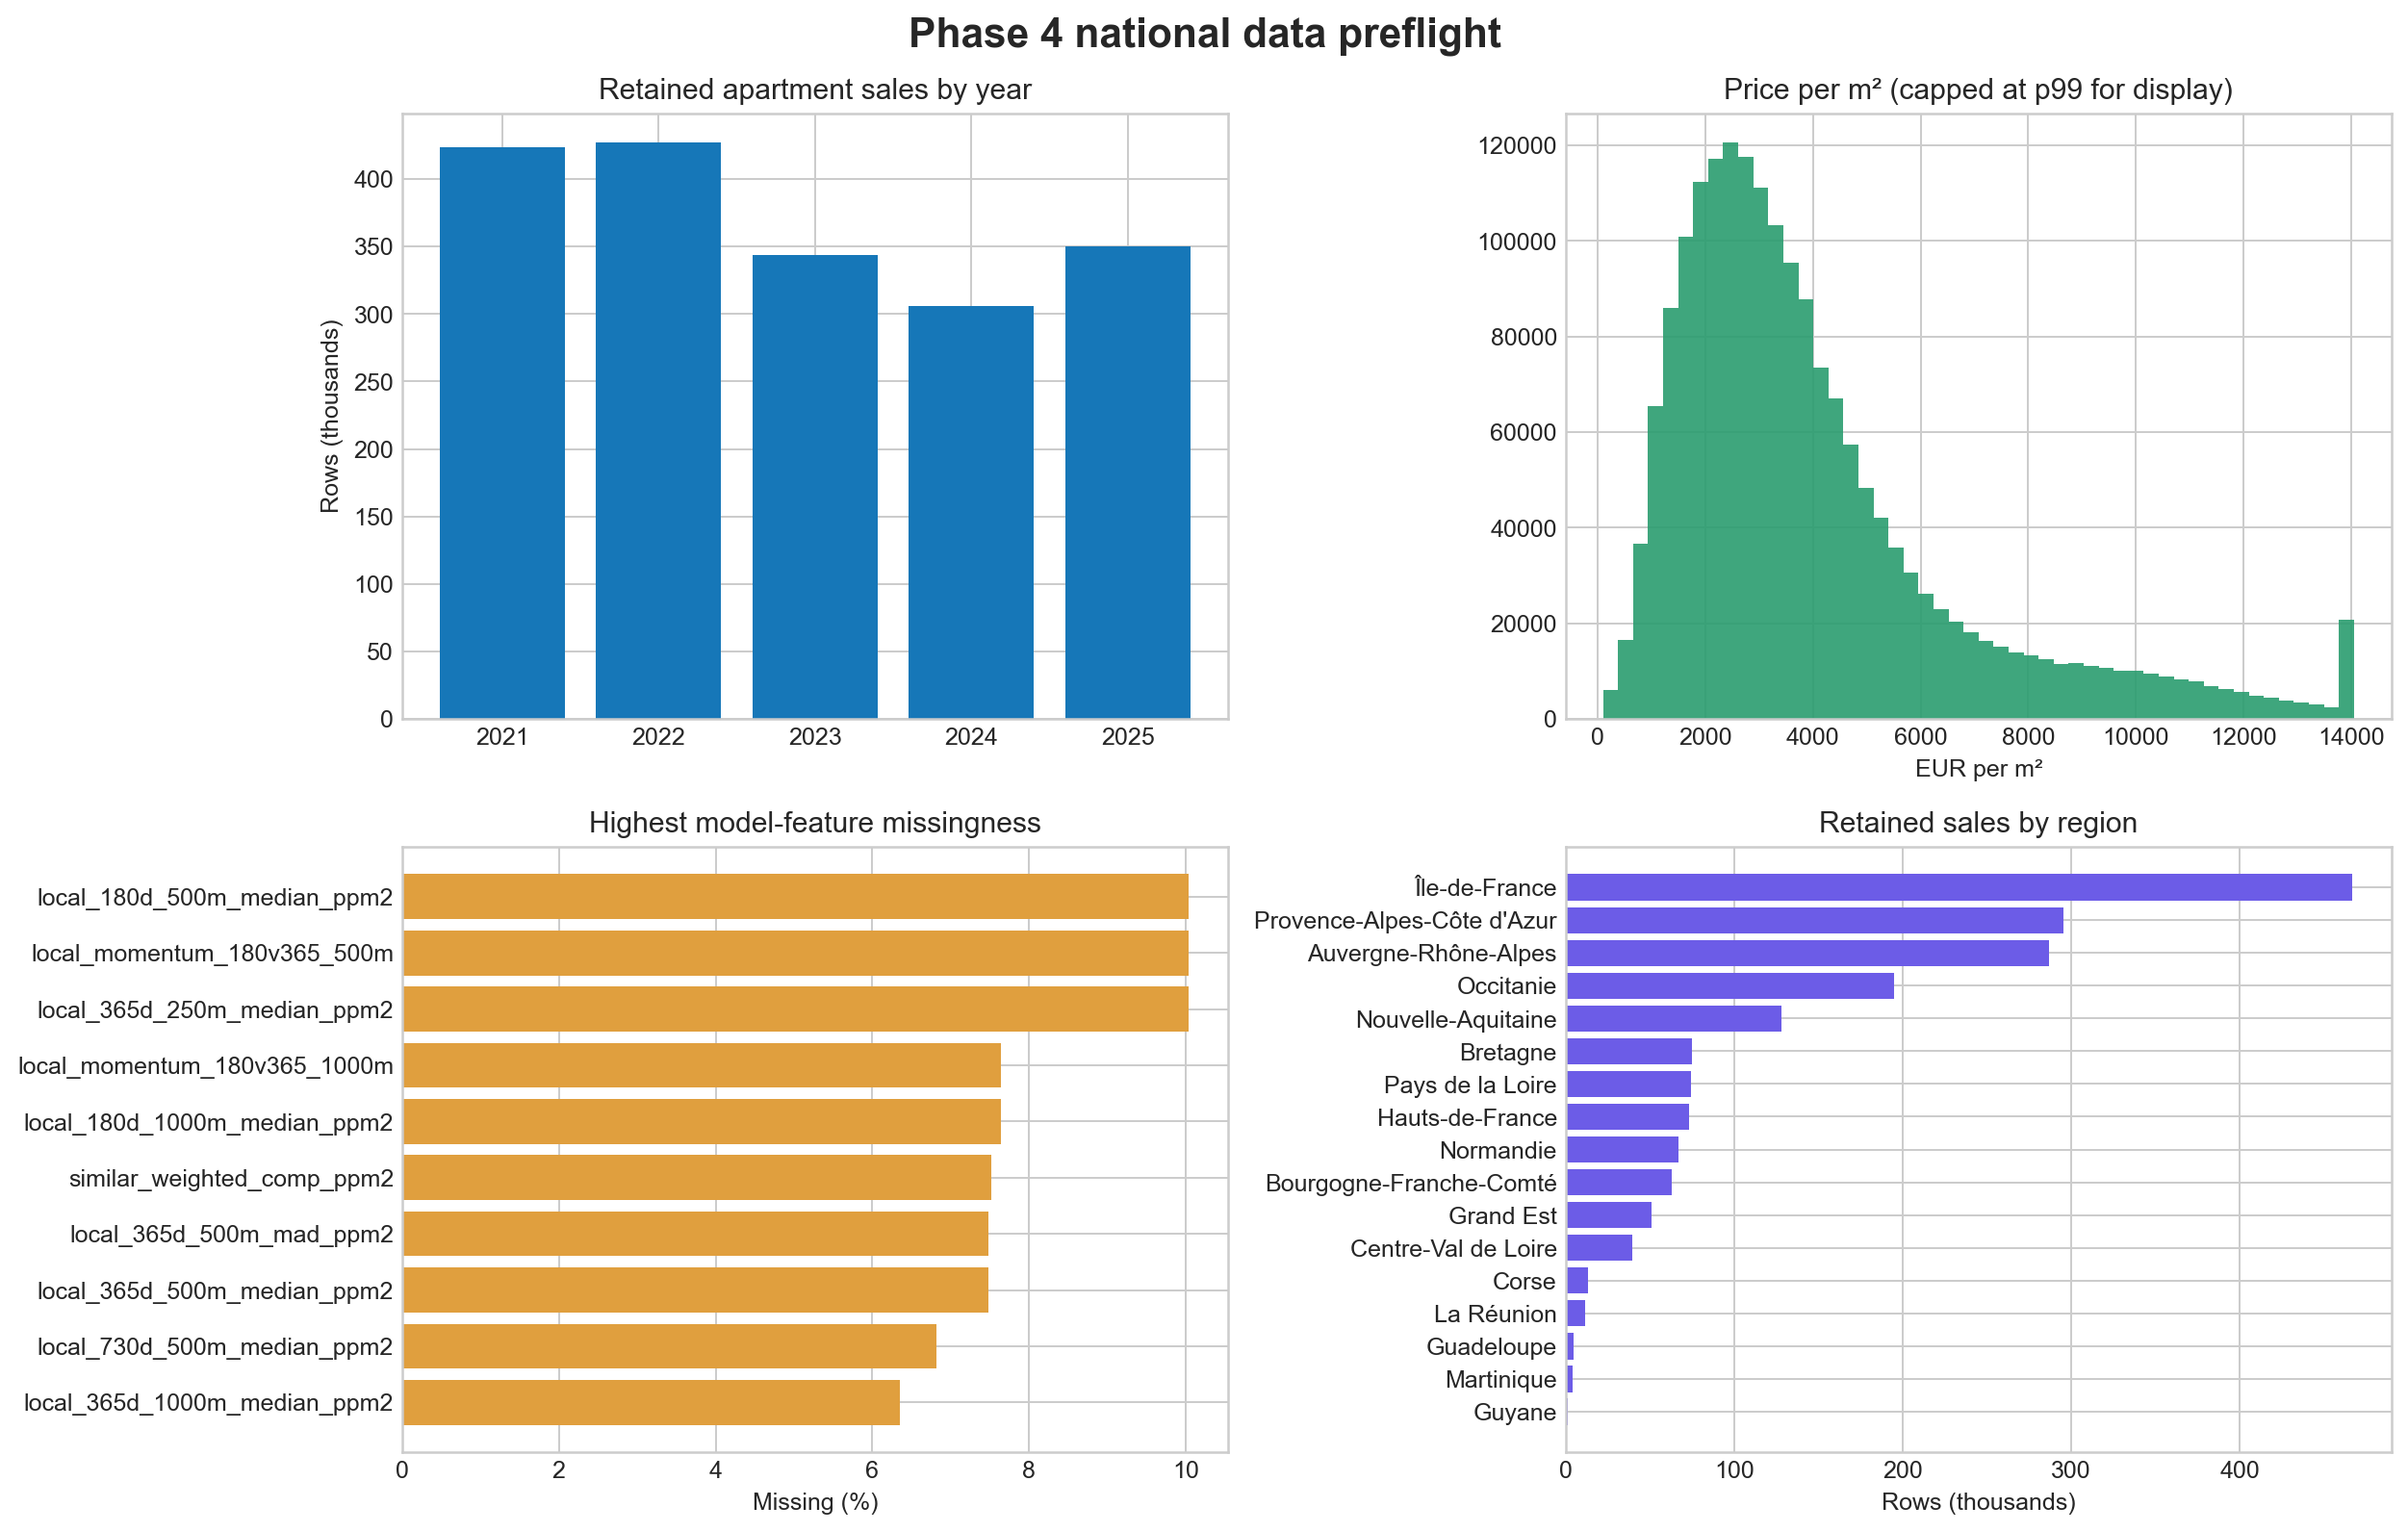
\includegraphics[width=\textwidth]{phase4_preflight_data_audit.png}
\caption{National pre-training audit: annual volume, price distribution, missingness and regional balance.}
\label{fig:preflight-audit}
\end{figure}


\begin{figure}[H]
\centering
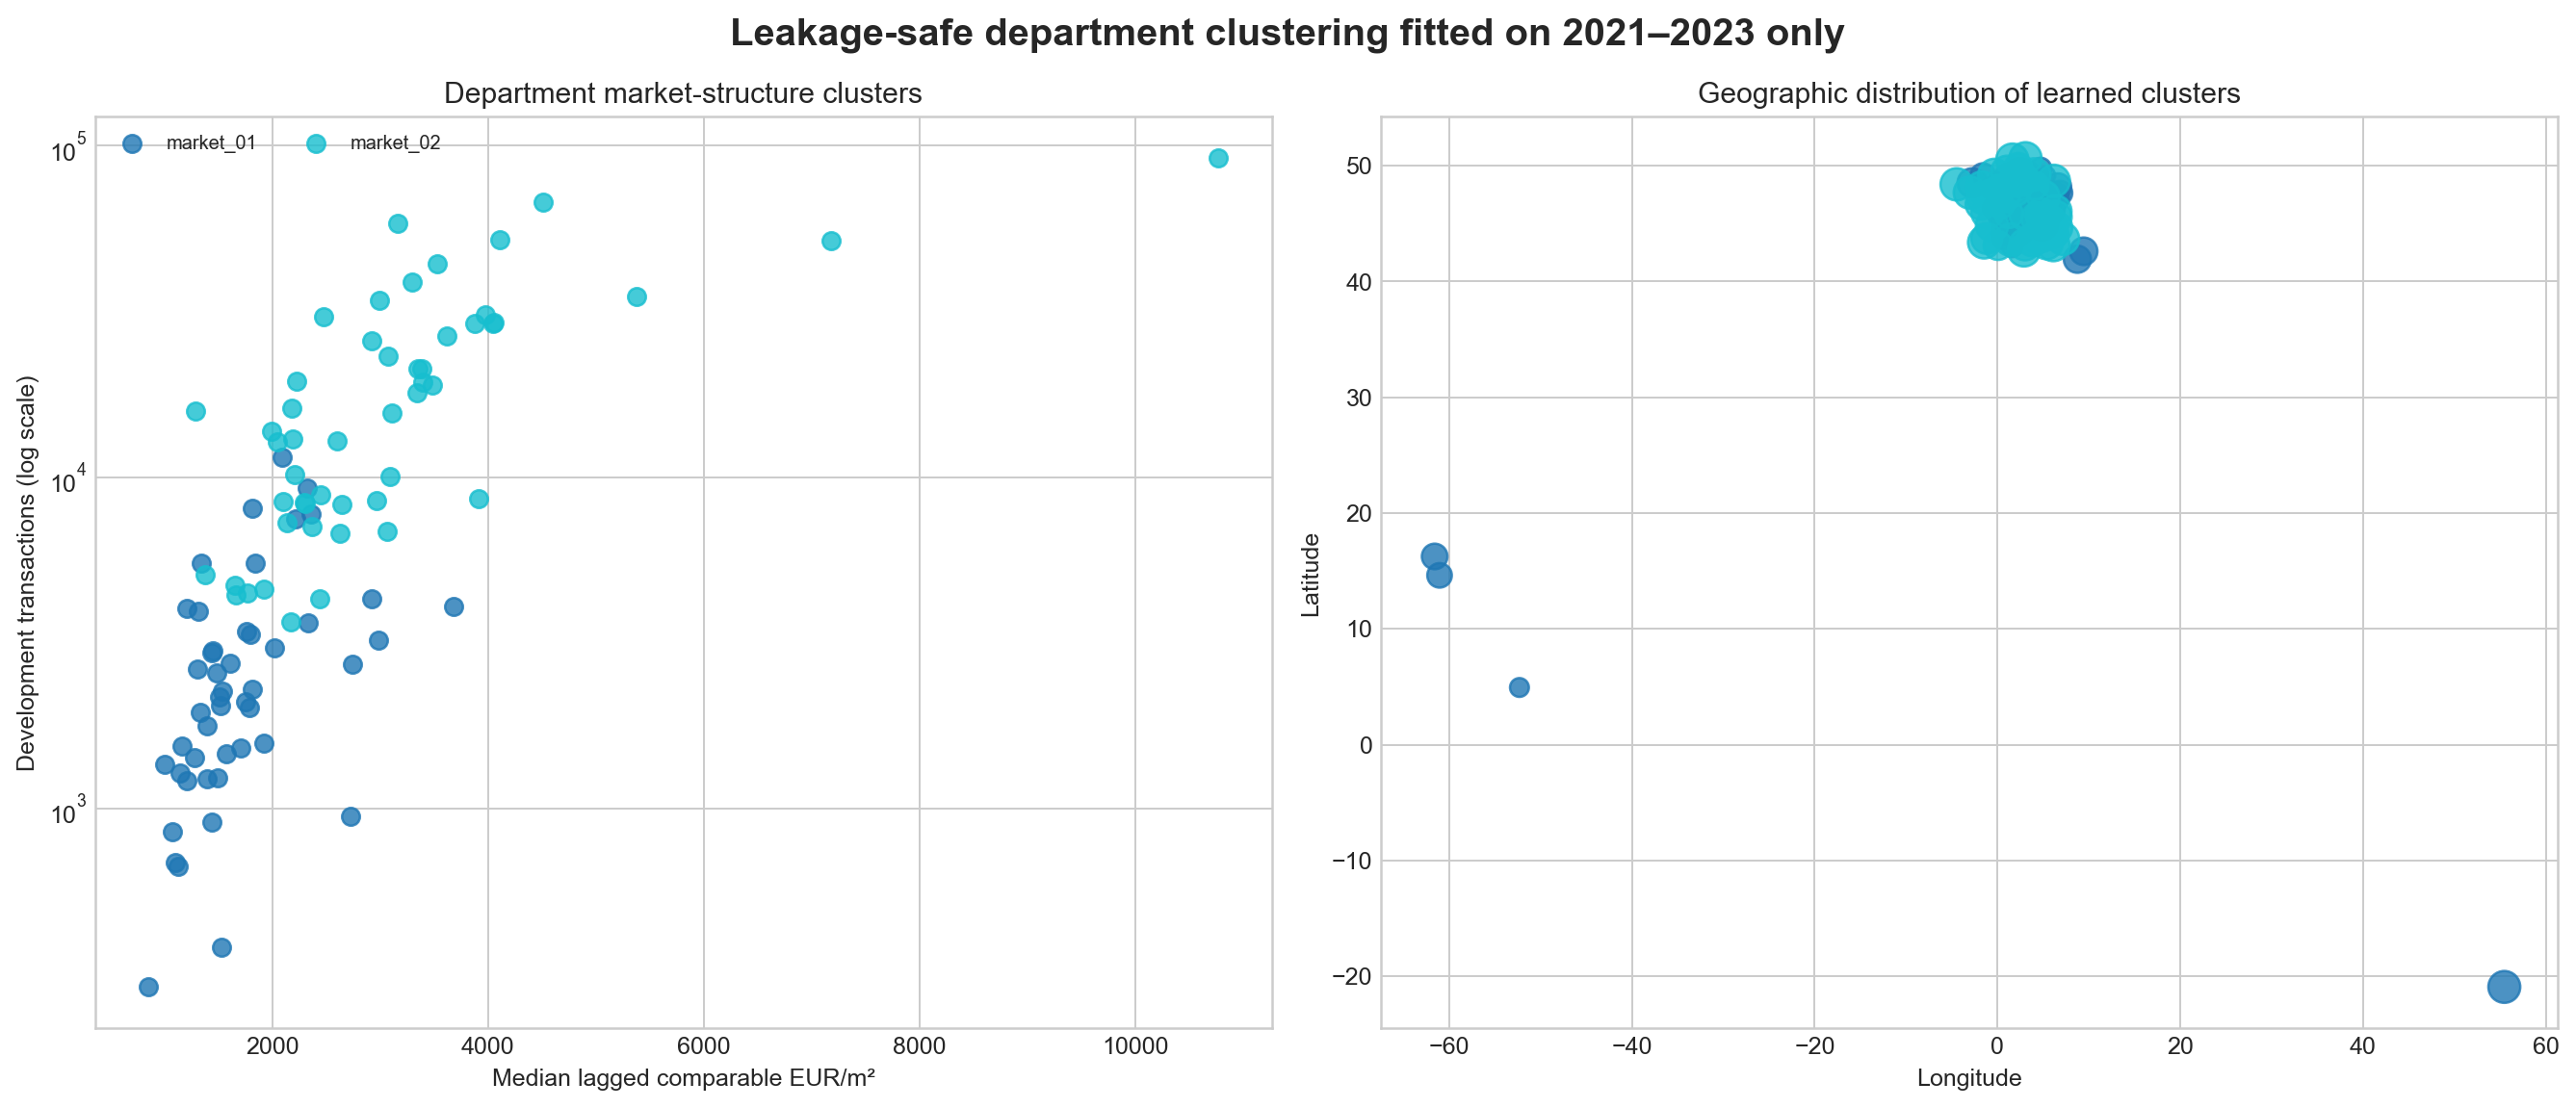
\includegraphics[width=\textwidth]{phase4_department_clusters.png}
\caption{Development-only department market-structure clusters and their geographic distribution.}
\label{fig:department-clusters}
\end{figure}



Development uses 2021--2023. Two predeclared CatBoost configurations are each
evaluated with and without the market-cluster feature on 2024; no 2025 outcome
participates in selection. The winner is
refitted through 2024 and evaluated once on 2025. Only after evaluation is the
production model refitted on all 2021--2025 observations.


\begin{table}[H]
\centering
\caption{CatBoost candidate performance on the 2024 selection cohort.}
\begin{tabularx}{\textwidth}{cXcrrrr}
\toprule
Candidate & Configuration & Cluster & Clipped & MAE & MdAPE & Within $\pm20\%$ \\
\midrule
1 & depth=8, loss=MAE, l2=8.0 & no & 0 & EUR 42,147 & 13.75\% & 65.55\% \\
3 & depth=8, loss=MAE, l2=8.0 & yes & 0 & EUR 42,161 & 13.74\% & 65.57\% \\
4 & depth=9, loss=Huber:delta=1.0, l2=10.0 & yes & 111,119 & EUR 1,544,040 & 56.52\% & 22.83\% \\
2 & depth=9, loss=Huber:delta=1.0, l2=10.0 & no & 201,487 & EUR 6,031,220 & 3289.83\% & 14.88\% \\
\bottomrule
\end{tabularx}
\end{table}


The Huber candidates generated extreme inverse-log outputs. The registered transaction-value bounds prevented non-finite metrics (candidate 2: 201,487, candidate 4: 111,119 clipped predictions), and their resulting validation errors rejected them from selection.

The objective is fitted to $\log(1+y)$ and transformed back to non-negative
euros. The benchmark baseline calculates median historical price per square
metre by postcode and falls back successively to commune, department, region
and national median. Every lookup is learned exclusively from the corresponding
training period.

\subsection{Metrics and paired uncertainty}

The report publishes MAE, RMSE, $R^2$, MAPE, median absolute percentage error
and hit rates within $\pm10\%$ and $\pm20\%$. Because model and baseline predict
the same transactions, uncertainty is estimated from paired absolute-error
differences. A deterministic bootstrap uses 300 repetitions and at most 250,000
test rows to bound memory. The exact sample size is stored in the benchmark JSON.

\section{Frozen national benchmark}


\begin{table}[H]
\centering
\caption{Frozen 2025 national benchmark on identical apartment transactions.}
\label{tab:national-benchmark}
\begin{tabular}{lrrrr}
\toprule
Method & MAE & RMSE & MdAPE & Within $\pm20\%$ \\
\midrule
Phase 4 CatBoost & EUR 41,936 & EUR 92,375 & 13.50\% & 66.97\% \\
Hierarchical median baseline & EUR 52,894 & EUR 108,830 & 18.37\% & 53.65\% \\
\bottomrule
\end{tabular}
\end{table}

The paired MAE reduction is EUR 10,957;
its deterministic paired-bootstrap 95\% interval is EUR 10,763--11,114.


\section{Territorial robustness}

Raw euro MAE is expected to be higher in expensive markets. Regional assessment
therefore requires MdAPE, hit rates, $R^2$ and sample size beside MAE. Department
rows require at least 100 test transactions; small segments are suppressed
rather than presented as stable estimates.


\begin{longtable}{p{4.1cm}rrrrr}
\caption{Frozen-test performance by region.}\label{tab:regions}\\
\toprule
Region & Rows & MAE & MdAPE & Within $\pm20\%$ & $R^2$ \\
\midrule
\endfirsthead
\toprule
Region & Rows & MAE & MdAPE & Within $\pm20\%$ & $R^2$ \\
\midrule
\endhead
Guyane & 315 & EUR 19,966 & 9.22\% & 80.63\% & 0.4994 \\
Centre-Val de Loire & 7,583 & EUR 21,840 & 13.68\% & 66.58\% & 0.7694 \\
Grand Est & 9,357 & EUR 24,482 & 16.37\% & 58.56\% & 0.7401 \\
Bourgogne-Franche-Comté & 11,843 & EUR 25,396 & 16.72\% & 58.13\% & 0.7188 \\
La Réunion & 2,006 & EUR 26,674 & 12.34\% & 69.49\% & 0.8030 \\
Normandie & 12,495 & EUR 27,043 & 14.22\% & 64.66\% & 0.7758 \\
Hauts-de-France & 13,583 & EUR 27,640 & 13.38\% & 67.53\% & 0.7954 \\
Occitanie & 37,205 & EUR 27,735 & 13.91\% & 65.27\% & 0.7473 \\
Pays de la Loire & 14,165 & EUR 29,952 & 12.79\% & 69.22\% & 0.7783 \\
Bretagne & 14,159 & EUR 30,070 & 12.64\% & 70.00\% & 0.7033 \\
Martinique & 727 & EUR 30,893 & 14.17\% & 64.24\% & 0.6421 \\
Guadeloupe & 801 & EUR 32,700 & 14.75\% & 62.92\% & 0.7218 \\
Nouvelle-Aquitaine & 24,590 & EUR 33,378 & 12.85\% & 68.41\% & 0.7878 \\
Auvergne-Rhône-Alpes & 53,825 & EUR 37,479 & 14.36\% & 64.55\% & 0.8171 \\
Corse & 2,596 & EUR 47,649 & 16.12\% & 59.05\% & 0.6277 \\
Provence-Alpes-Côte d'Azur & 56,352 & EUR 49,751 & 15.34\% & 61.36\% & 0.7395 \\
Île-de-France & 88,797 & EUR 62,277 & 11.71\% & 73.98\% & 0.8533 \\
\bottomrule
\end{longtable}


\section{Calibration and uncertainty}

The empirical 90\% interval uses 2024 target-to-prediction ratios. A region gets
its own calibration ratios only with at least 500 observations; otherwise it
inherits the national interval. Observed 2025 coverage evaluates temporal
transfer but is not a formal conditional guarantee for a specific apartment.

\section{Visual diagnostic suite}


\begin{figure}[H]
\centering
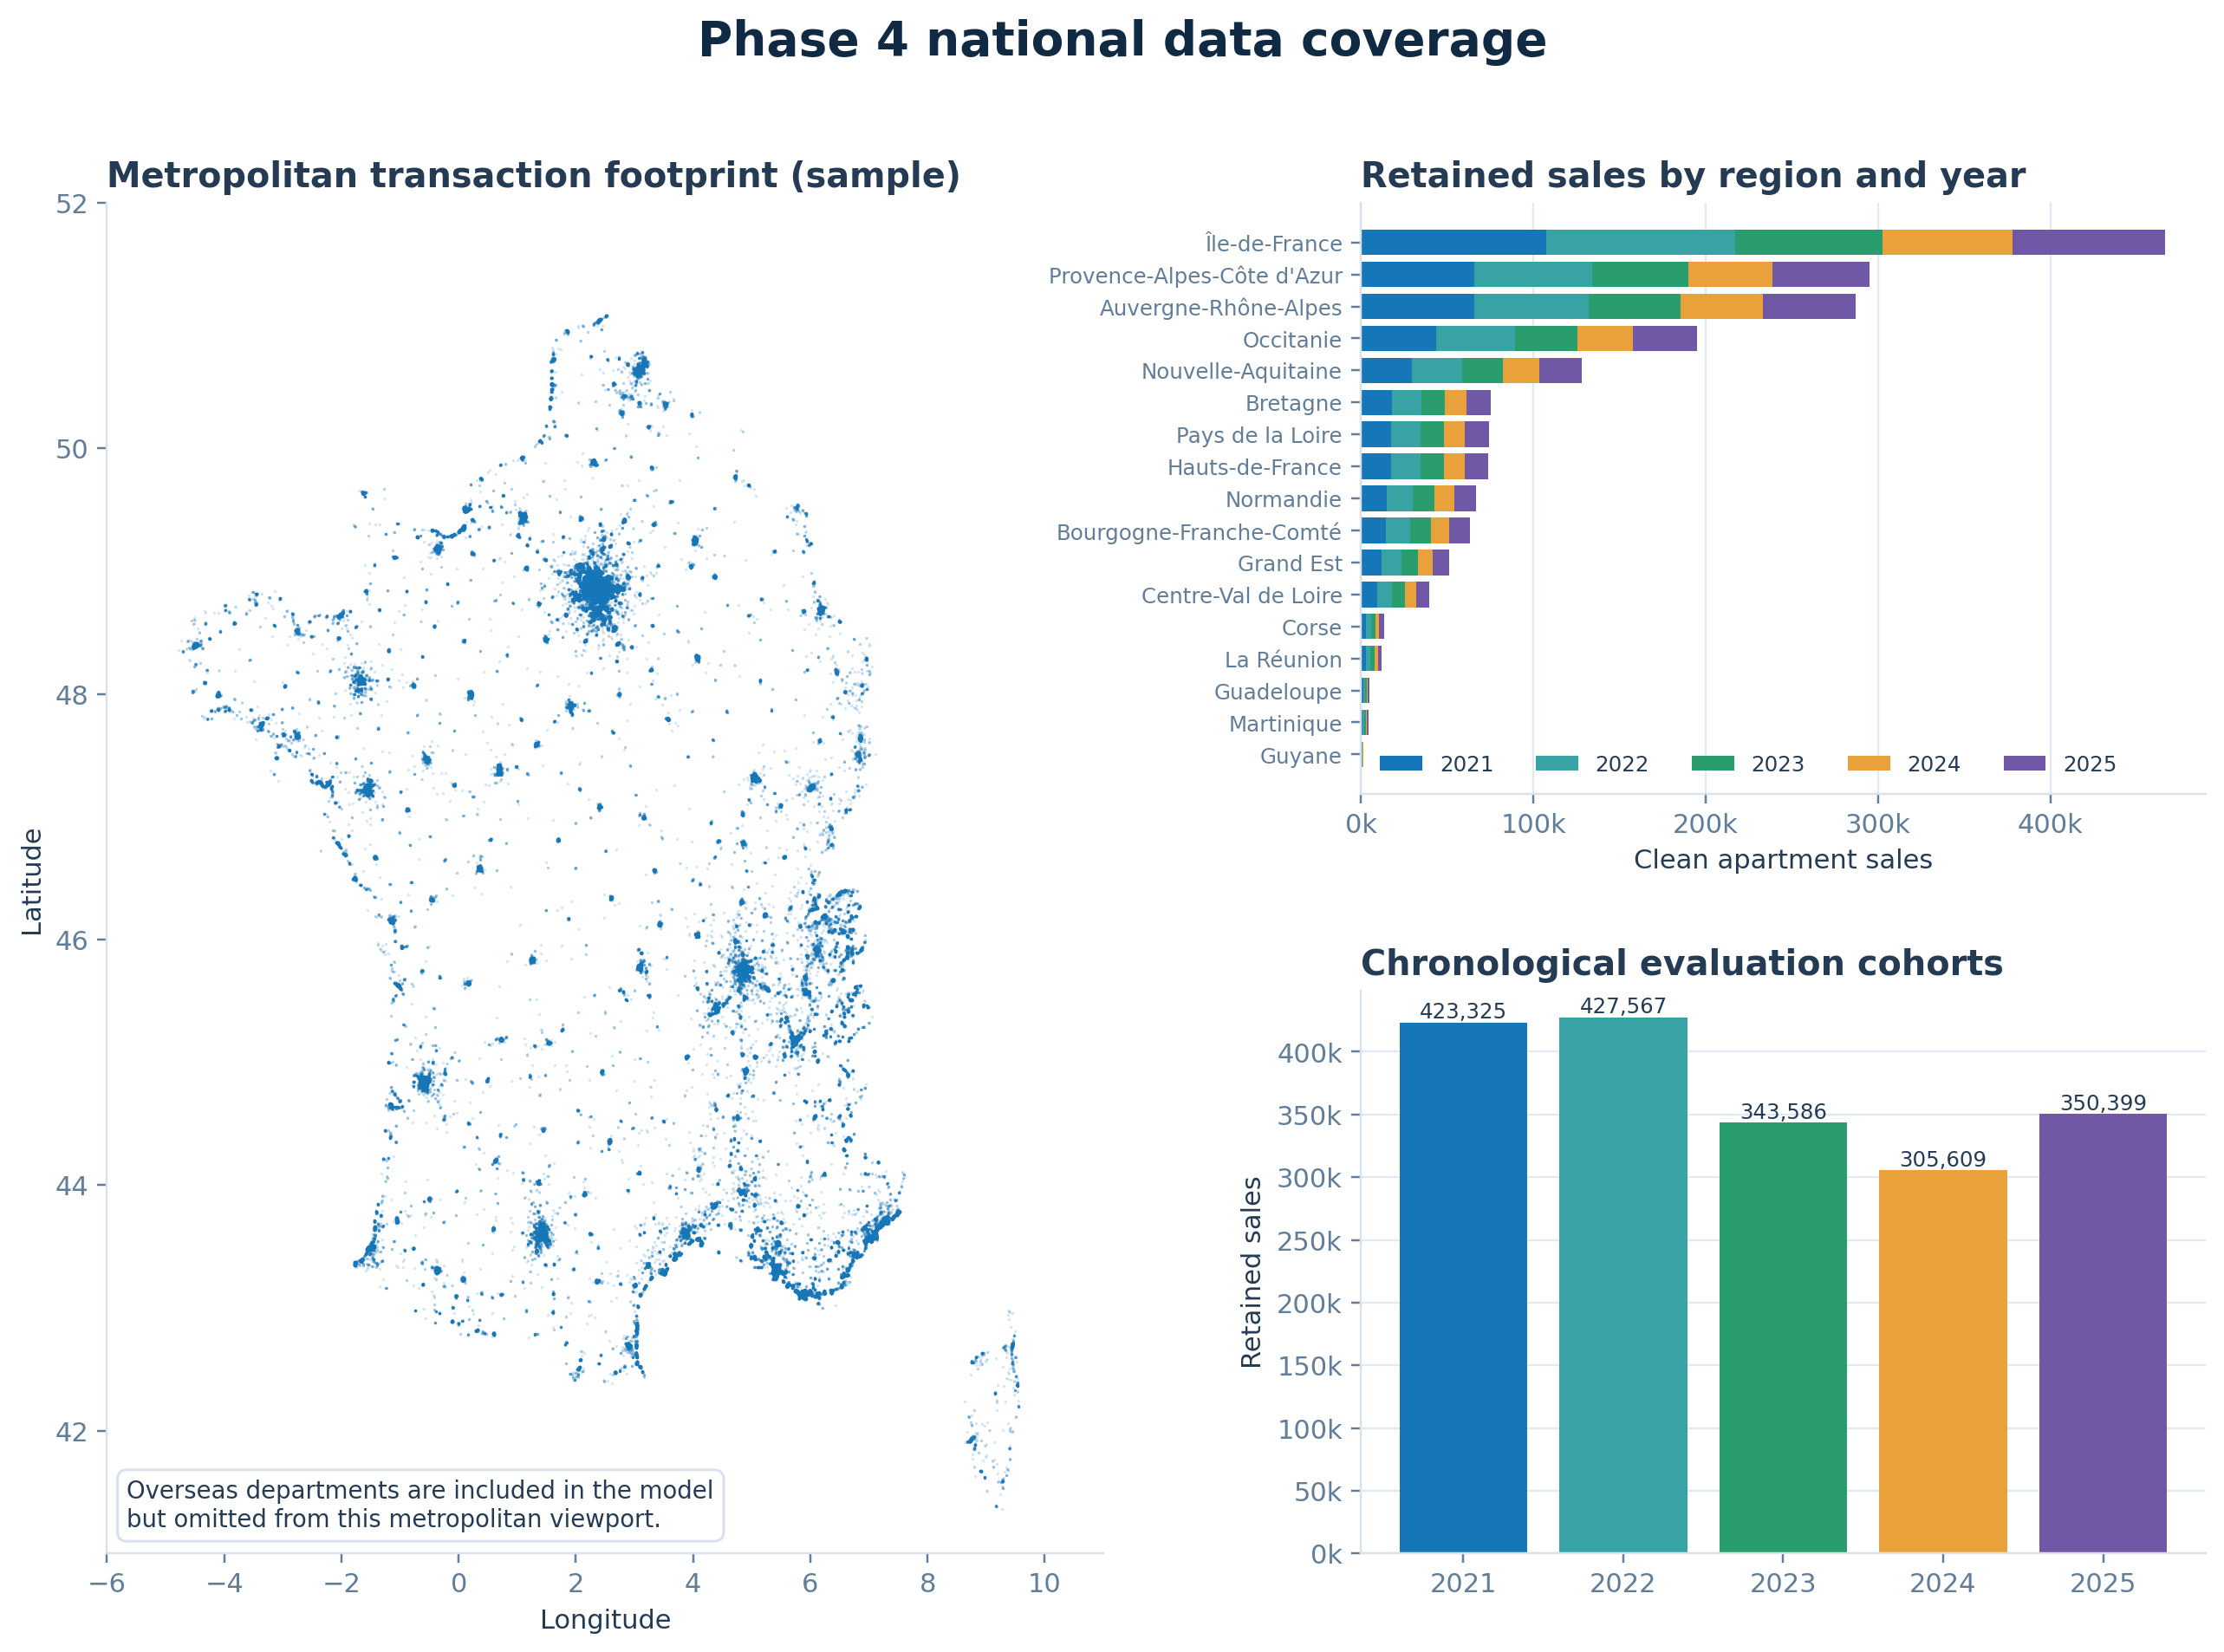
\includegraphics[width=\textwidth]{phase4_national_coverage.png}
\caption{National transaction footprint, retained sales by region and chronological cohorts.}
\label{fig:coverage}
\end{figure}


\begin{figure}[H]
\centering
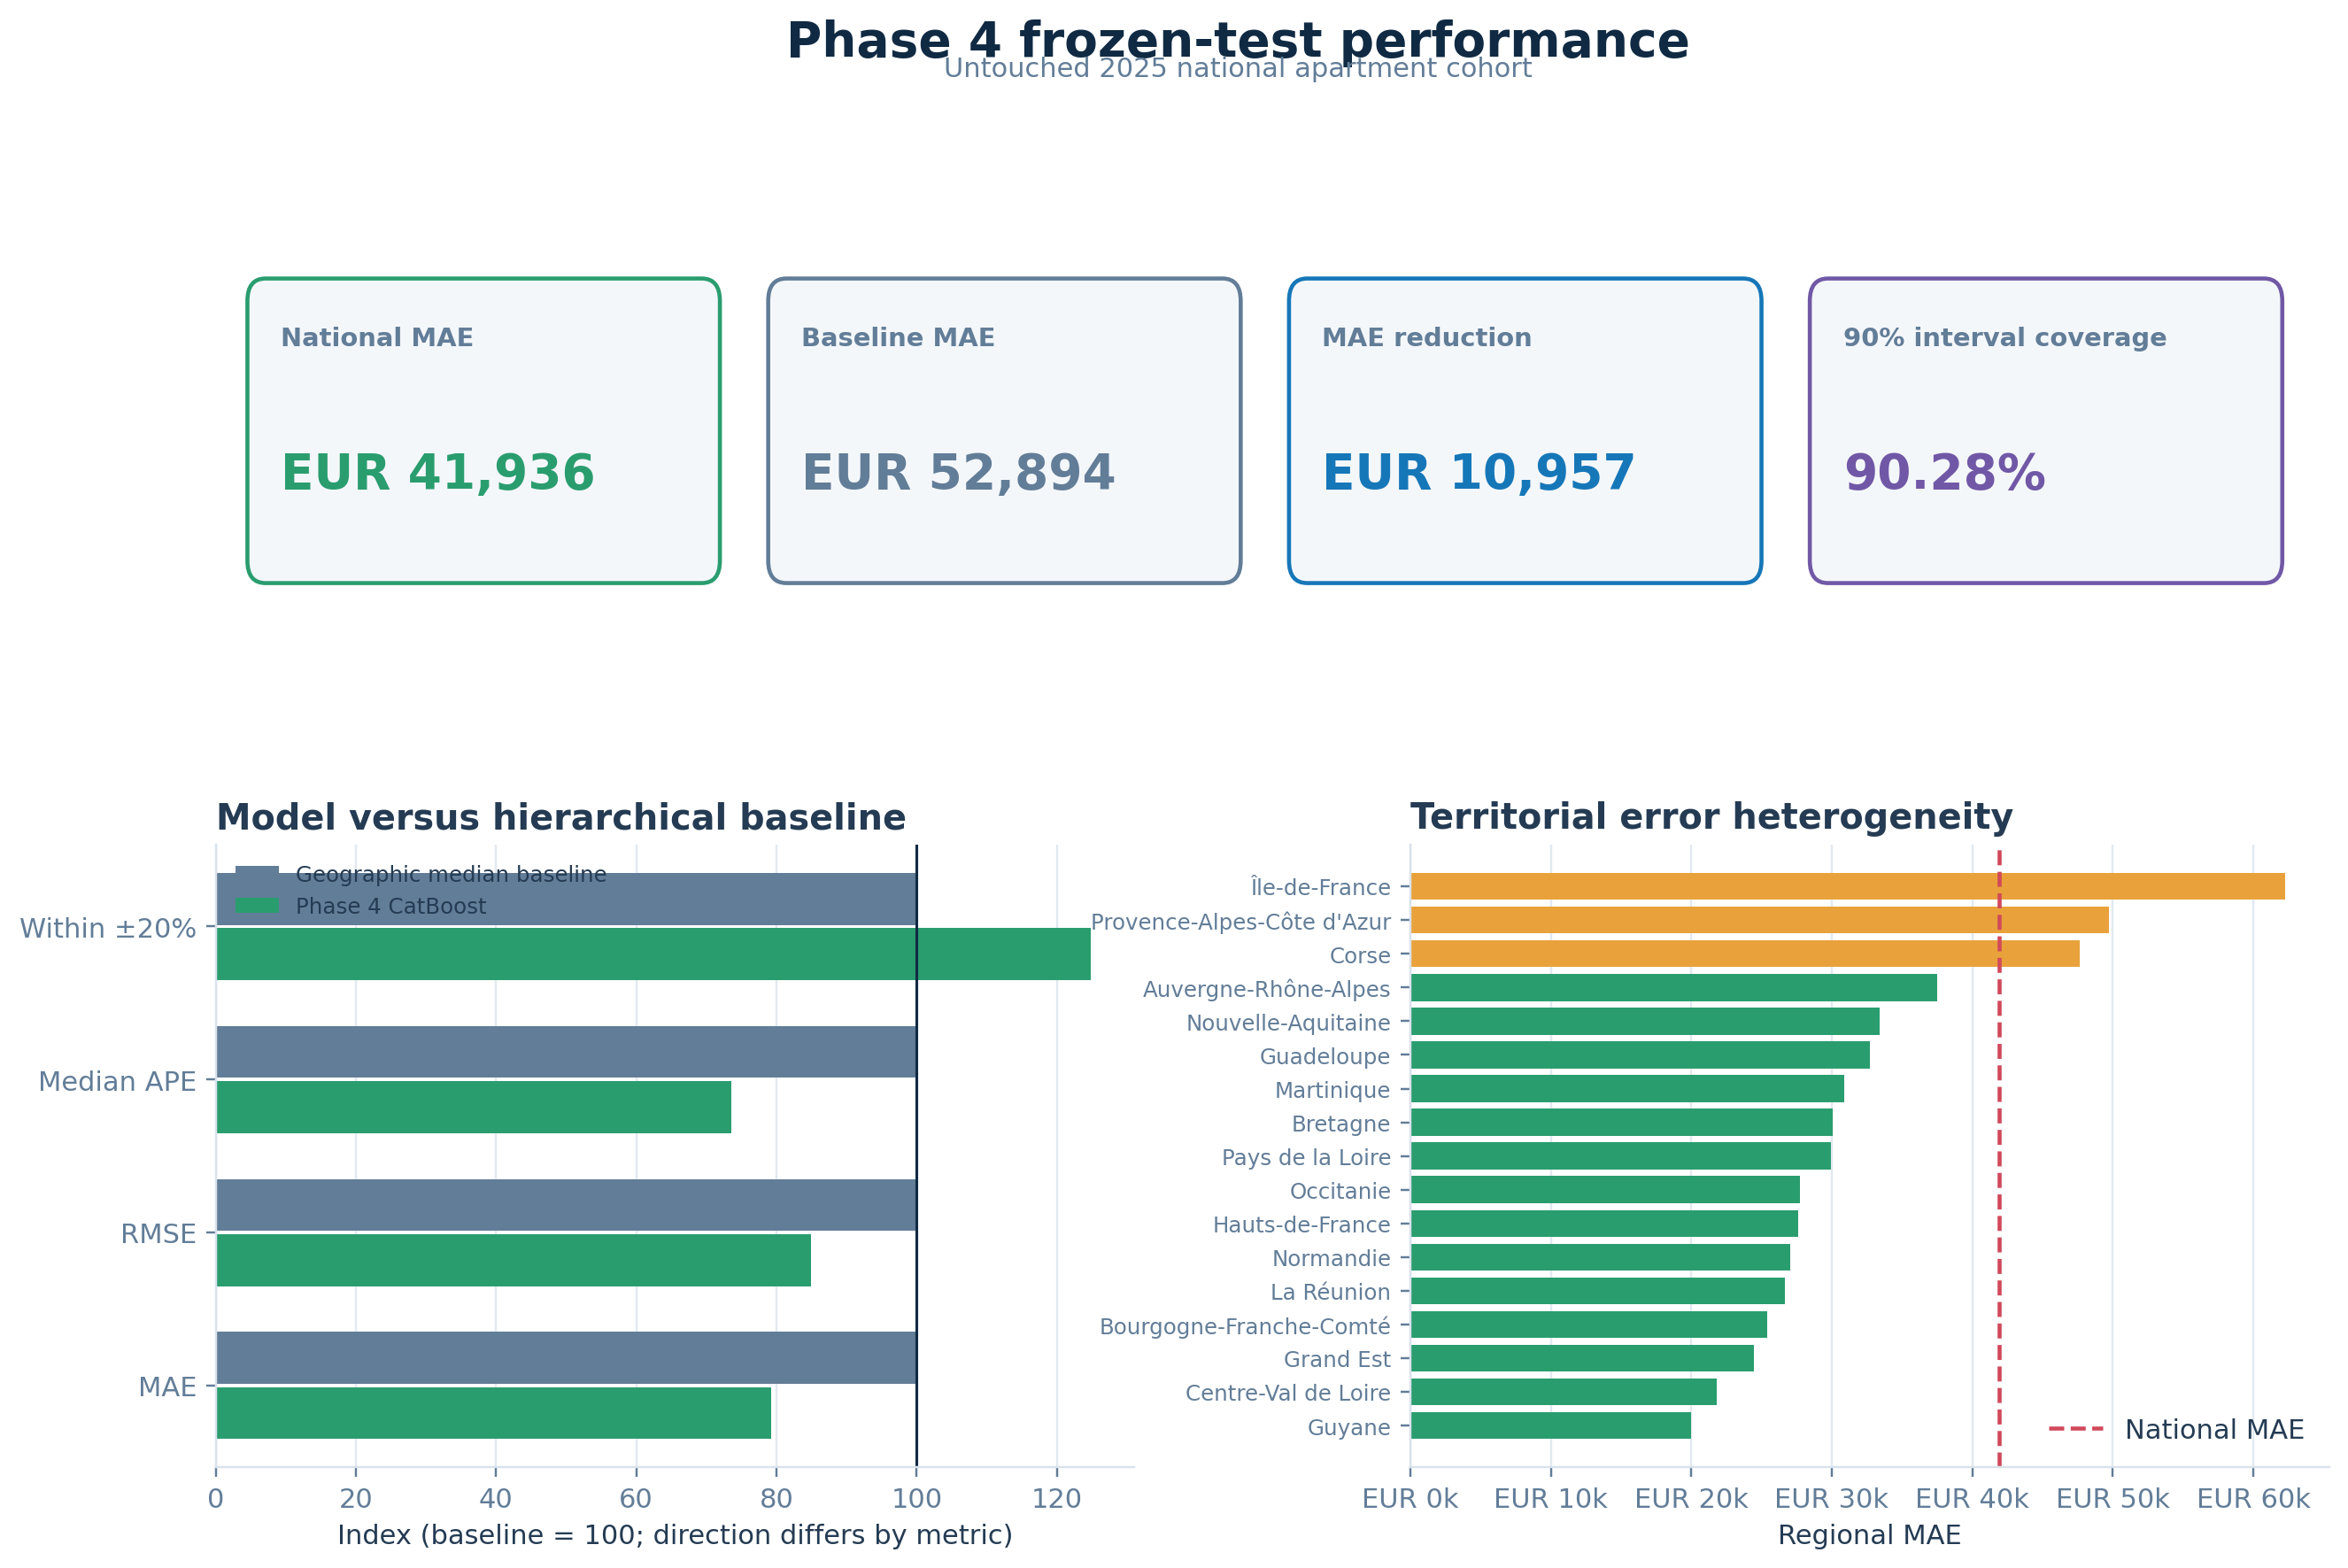
\includegraphics[width=\textwidth]{phase4_performance_dashboard.png}
\caption{Frozen-test model-versus-baseline benchmark and regional error heterogeneity.}
\label{fig:performance}
\end{figure}


\begin{figure}[H]
\centering
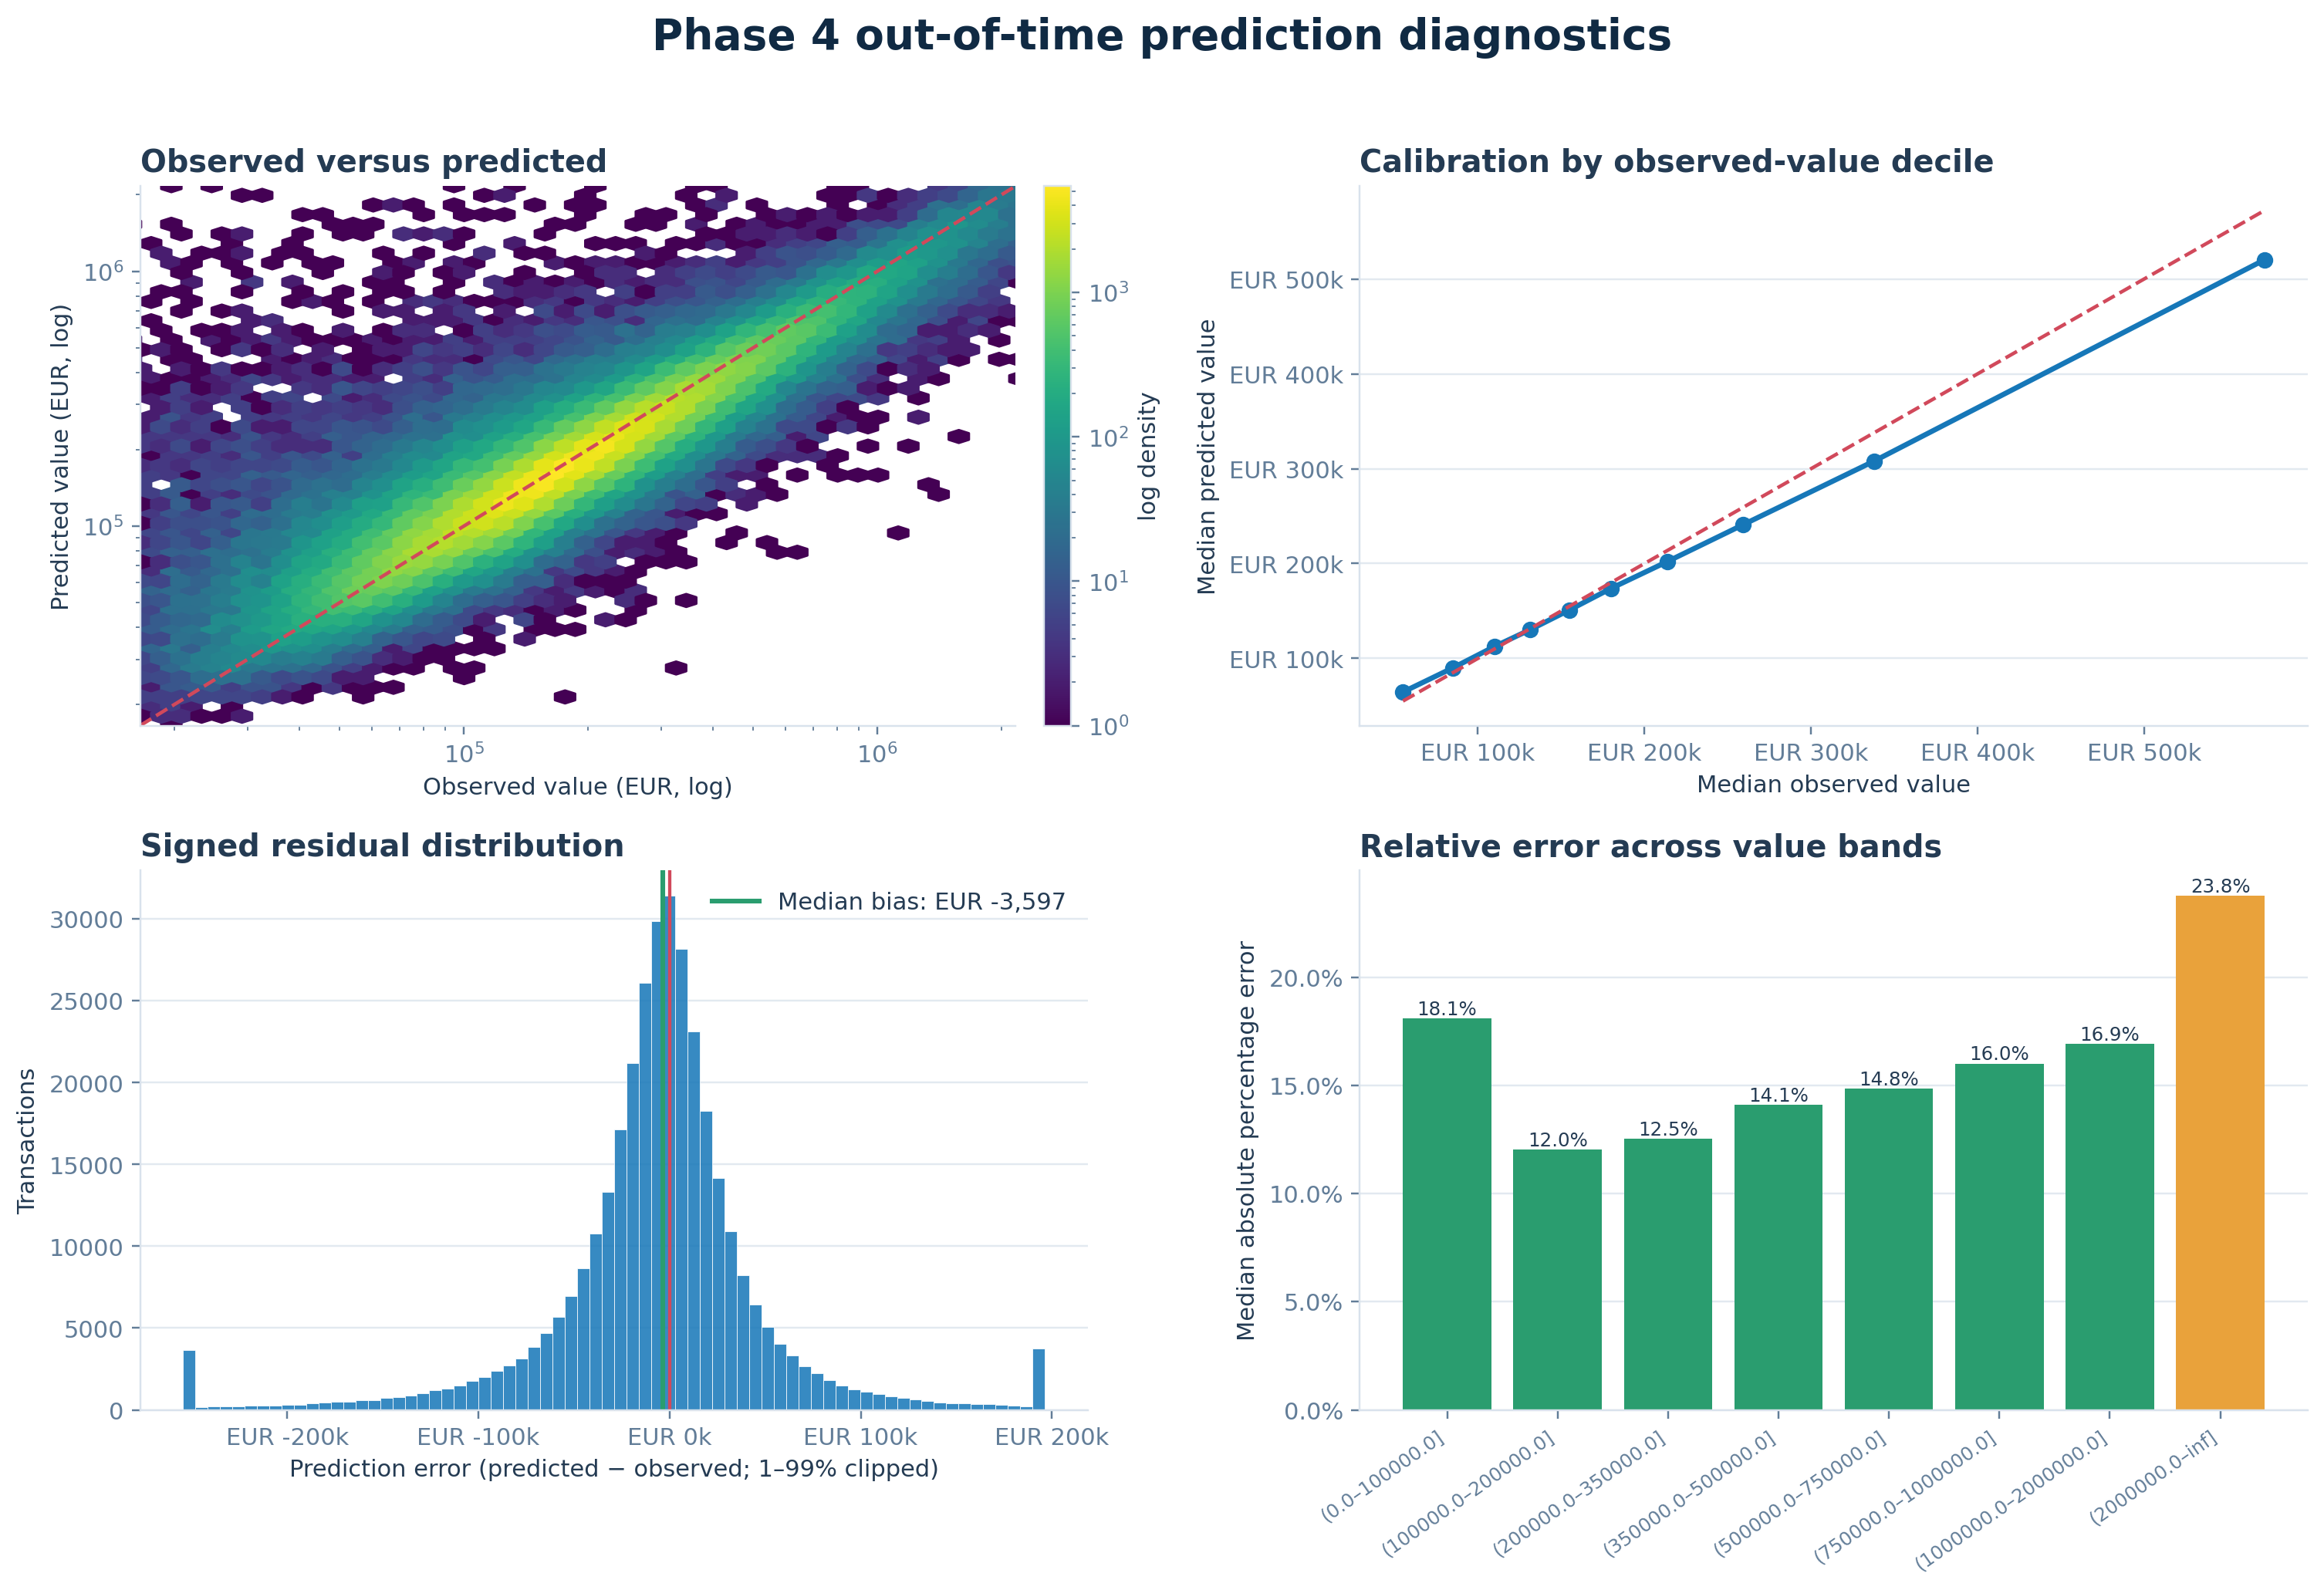
\includegraphics[width=\textwidth]{phase4_prediction_diagnostics.png}
\caption{Out-of-time calibration, residual and value-band diagnostics.}
\label{fig:diagnostics}
\end{figure}


\begin{figure}[H]
\centering
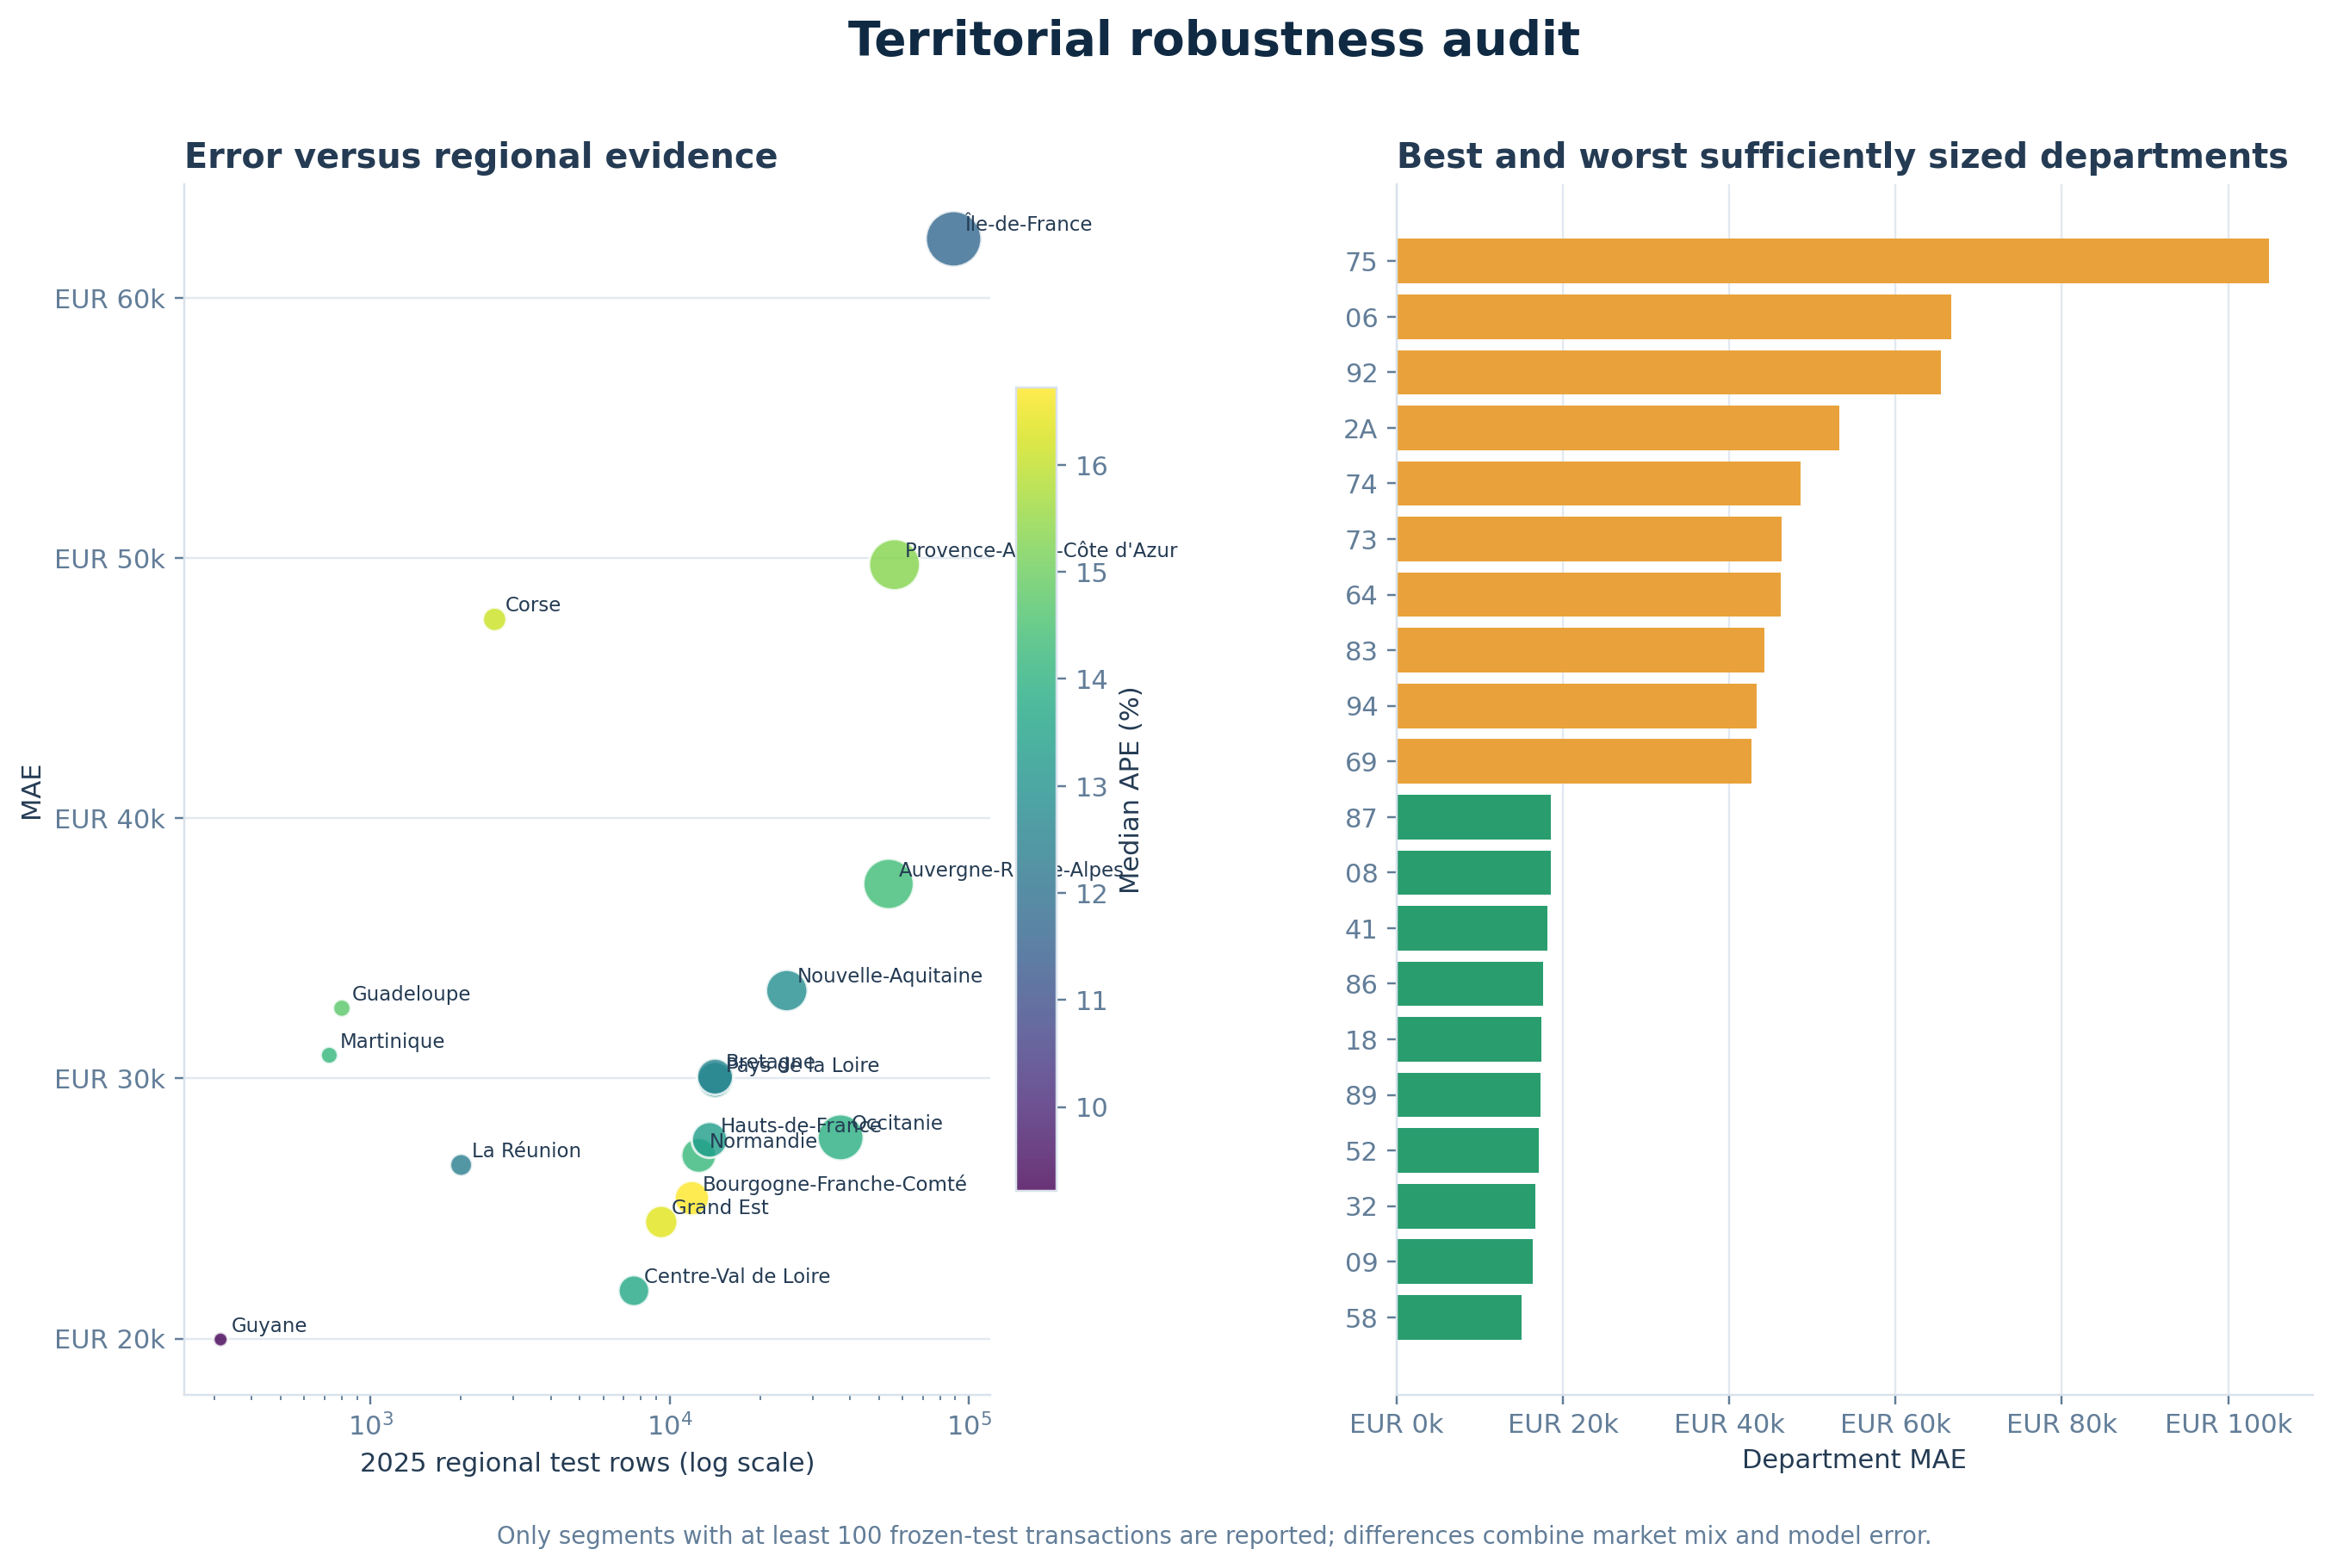
\includegraphics[width=\textwidth]{phase4_regional_performance.png}
\caption{Regional evidence and department-level robustness audit.}
\label{fig:regional}
\end{figure}


\begin{figure}[H]
\centering
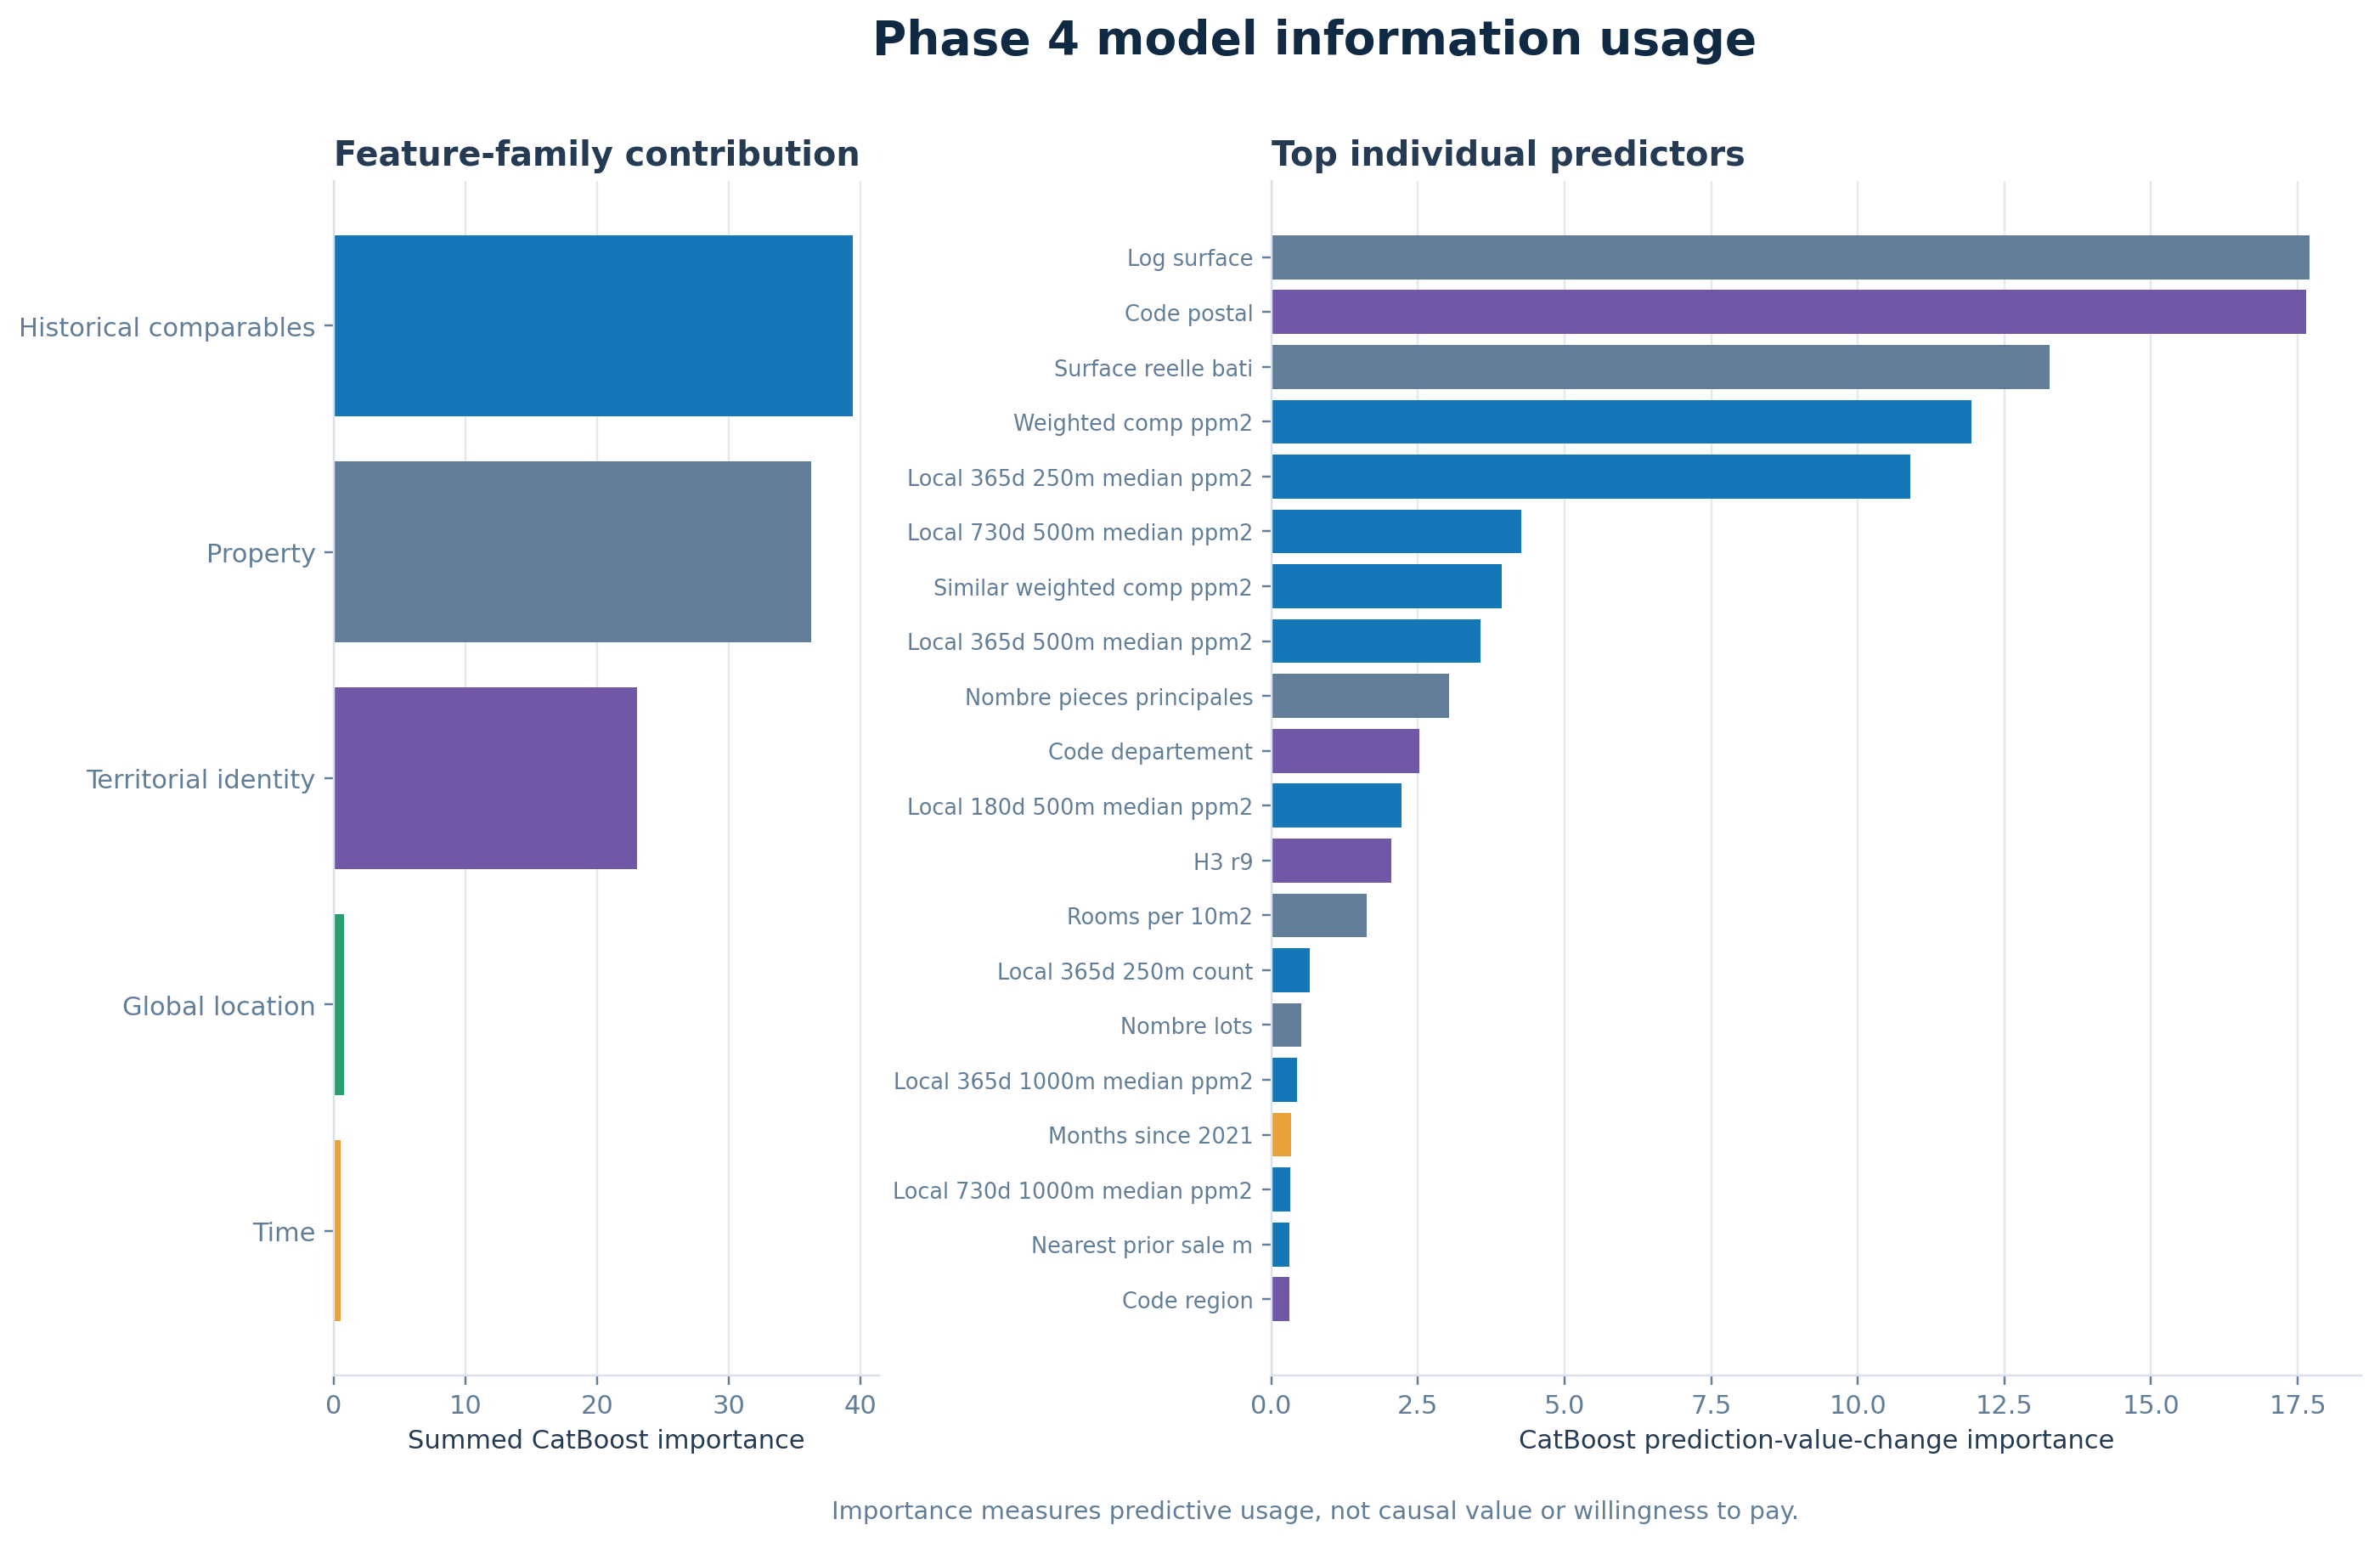
\includegraphics[width=\textwidth]{phase4_feature_importance.png}
\caption{CatBoost information usage by feature family and individual input.}
\label{fig:importance}
\end{figure}


\begin{figure}[H]
\centering
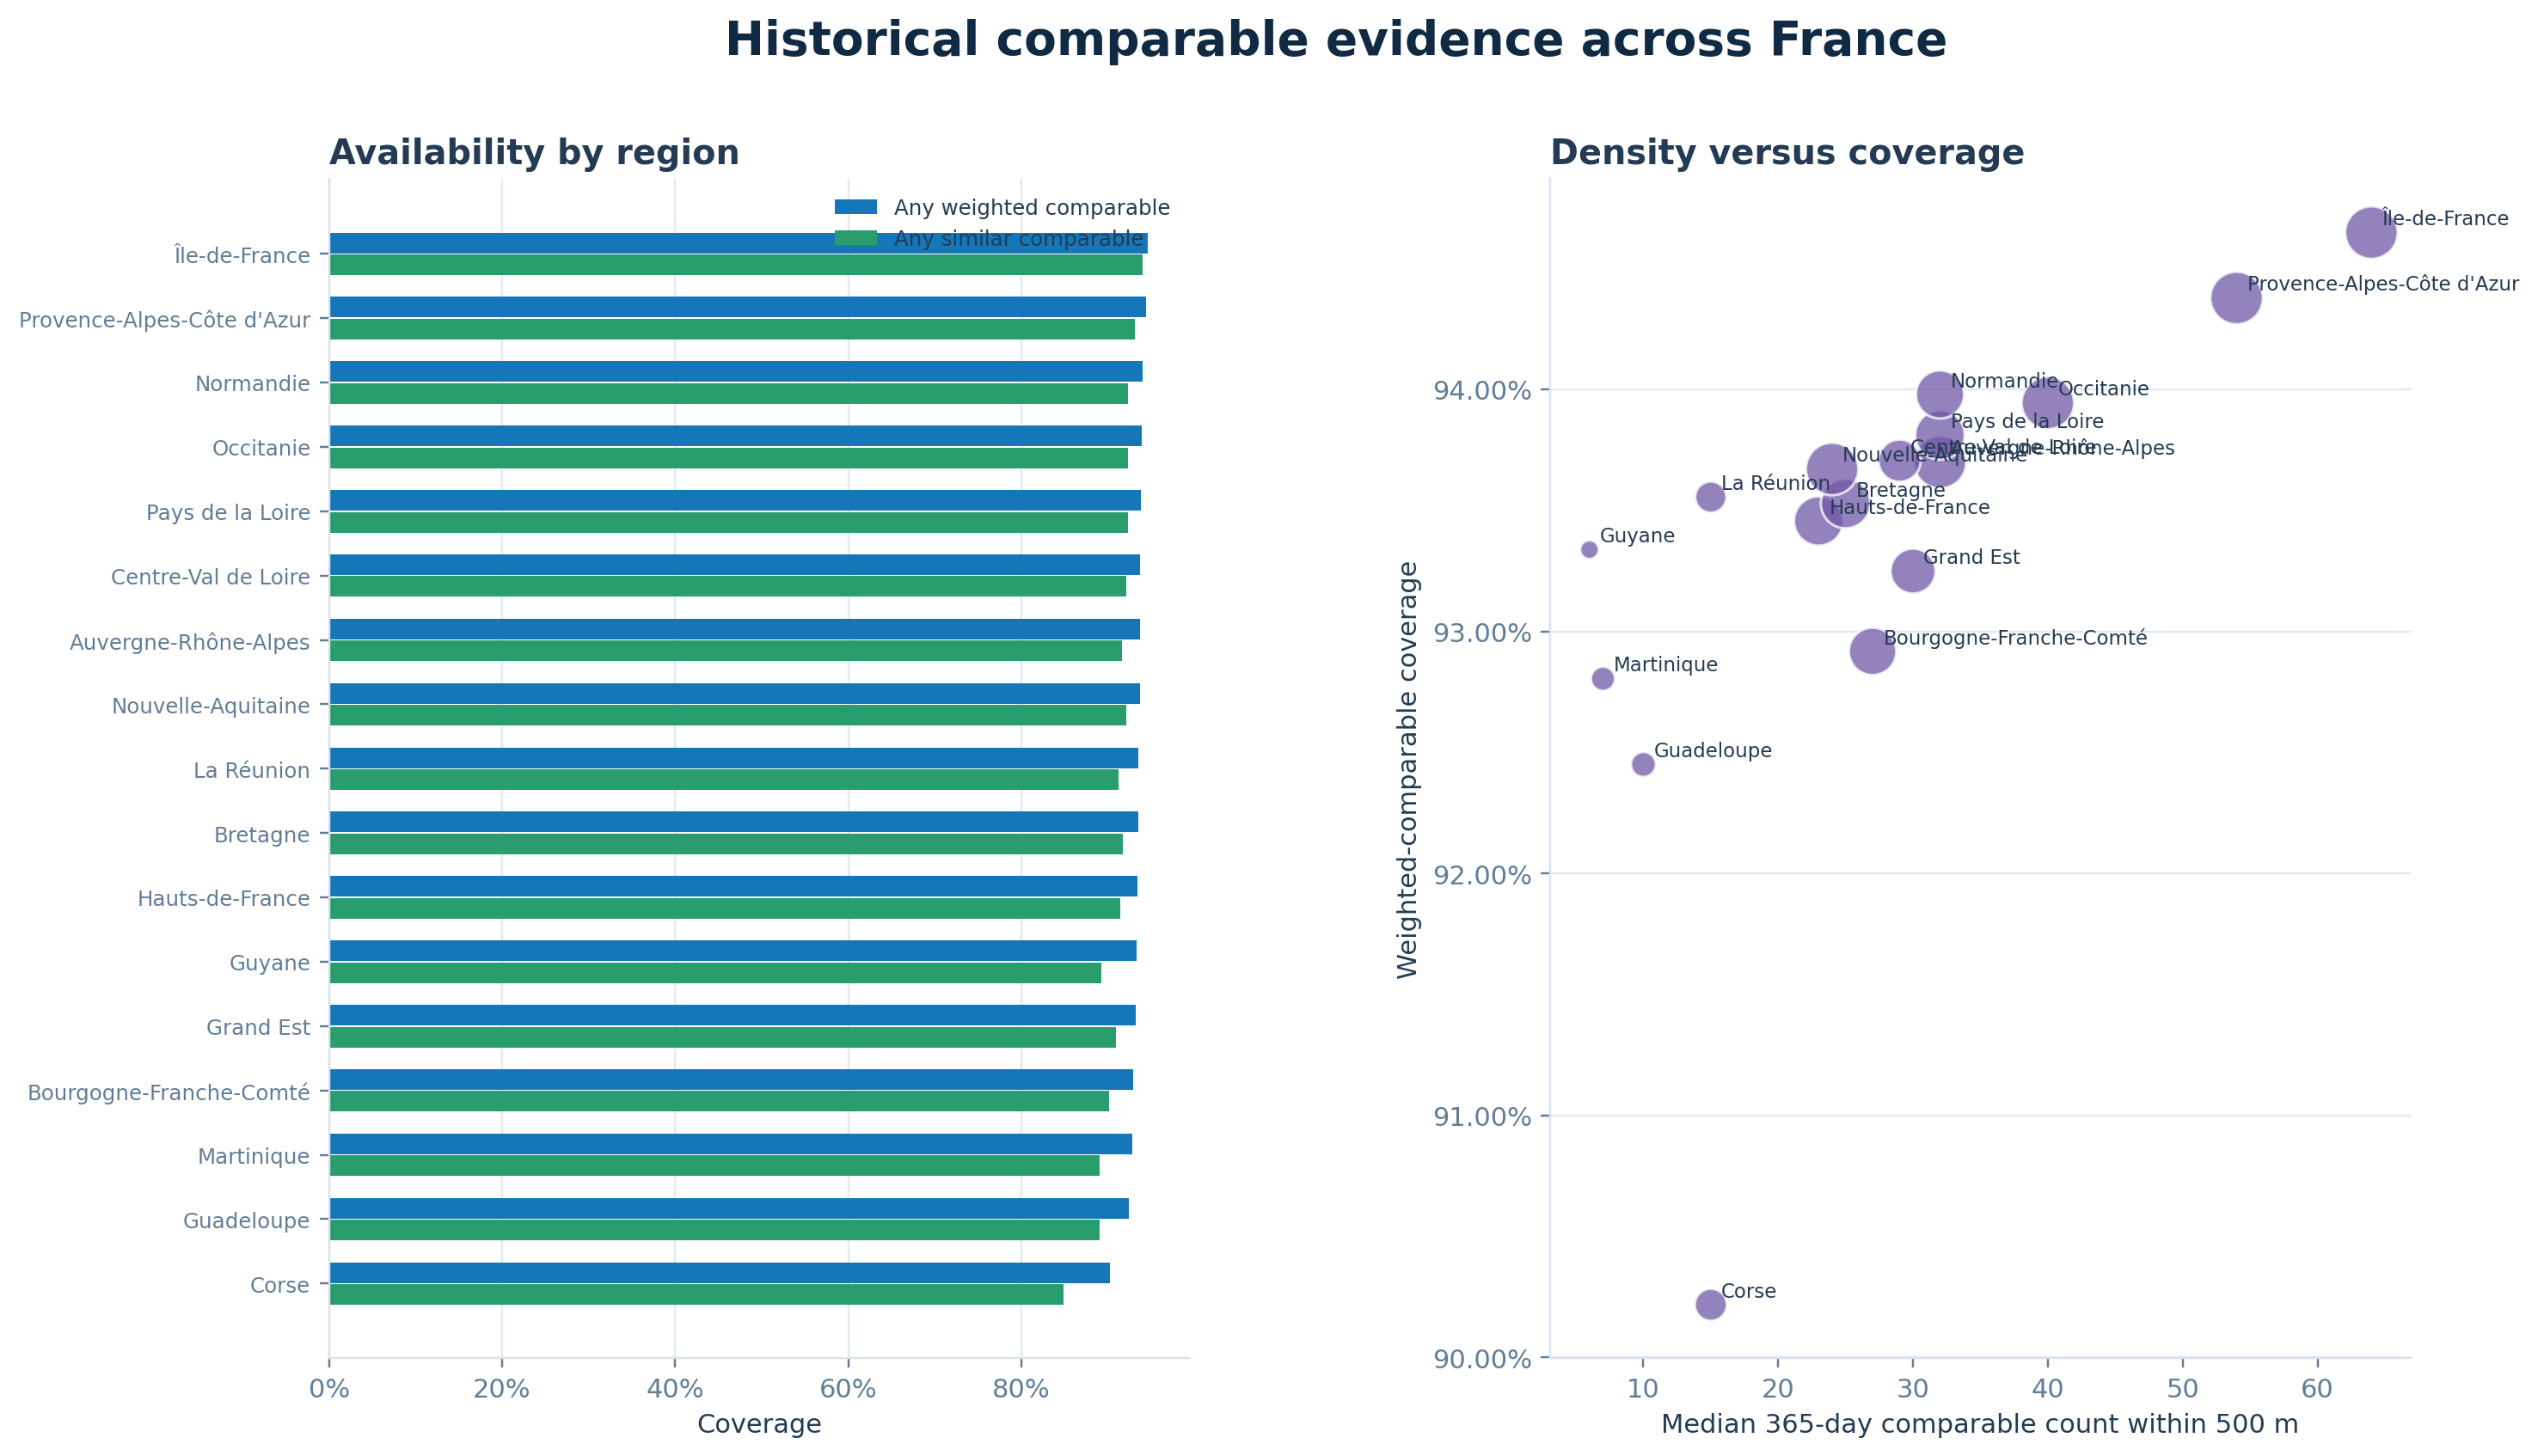
\includegraphics[width=\textwidth]{phase4_comparable_coverage.png}
\caption{Lagged comparable-sale availability and density by region.}
\label{fig:comparables}
\end{figure}


Figures are generated only from existing artifacts. Missing benchmark outputs
produce no placeholder chart and no synthetic metric. Feature importance records
predictive usage rather than a causal housing premium.

\section{Reproducibility and artifact inventory}

\begin{longtable}{p{5.8cm}lr}
\toprule
Artifact & Status & Bytes \\
\midrule
\endfirsthead
\toprule Artifact & Status & Bytes \\
\midrule
\endhead
Source manifest & available & 2,319 \\
Gold feature table & available & 340,479,232 \\
Feature quality report & available & 8,645 \\
Preflight summary & available & 2,931 \\
Department market clusters & available & 21,305 \\
Preflight Markdown report & available & 2,940 \\
Benchmark JSON & available & 7,425 \\
Validation trials & available & 817 \\
Benchmark comparison & available & 462 \\
Frozen predictions & available & 15,829,165 \\
Regional metrics & available & 1,399 \\
Department metrics & available & 5,795 \\
Feature importance & available & 1,778 \\
Production model & available & 497,458,679 \\
\bottomrule
\end{longtable}

\begin{verbatim}
python -m paris_avm.data.acquire_phase4
python -m paris_avm.features.phase4
python -m paris_avm.analysis.phase4_preflight
python -m paris_avm.modeling.benchmark_phase4
python -m paris_avm.visualization.phase4
python -m paris_avm.reporting.phase4
powershell -ExecutionPolicy Bypass -File .\docs\paper\compile_phase4.ps1
\end{verbatim}

\section{Limitations and responsible use}

\begin{itemize}[leftmargin=1.5em]
\item DVF omits condition, renovation, floor, elevator, view and occupancy.
\item Mutation value can bundle dependencies or transaction-specific rights.
\item Departments 57, 67, 68 and 976 are absent from the source.
\item Sparse submarkets may have weak comparable coverage and unstable errors.
\item Administrative/H3 identity is predictive context, not a causal estimate.
\item A 2025 holdout does not establish performance in 2026 or later markets.
\item The interval is empirical and marginal, not a certified property guarantee.
\item Predictions are not notarial valuations, lending decisions or investment advice.
\end{itemize}

\section{Conclusion}

Phase 4 defines a scalable and auditable path from a Paris research model to a
national France AVM. Its strongest contribution is the combination of global
geography, local point-in-time market evidence, chronological evaluation and
territorial reporting. In this empirical benchmark edition, claims remain limited to the
artifacts actually present. The completed frozen evaluation supports a national
2025 MAE of EUR 41,936 and a paired improvement of EUR
10,957 over the training-only baseline.
The empirical claims in this edition are generated directly from the registered
benchmark artifacts; limitations remain especially important for sparse territories
and for applications beyond the 2025 evaluation period.

\appendix
\section{Machine-readable deliverables}

The benchmark publishes JSON metrics, validation trials, a two-method comparison,
regional and department CSV tables, Parquet predictions with paired errors,
feature importance and a checksummed Joblib production bundle. The Markdown and
LaTeX reports consume these outputs without refitting or selecting a model.

\section{Source references}

\begin{itemize}[leftmargin=1.5em]
\item \href{https://www.data.gouv.fr/datasets/demandes-de-valeurs-foncieres-geolocalisees}{Geo-DVF dataset catalogue on data.gouv.fr}
\item \href{https://files.data.gouv.fr/geo-dvf/latest/csv/}{Geo-DVF annual file index}
\item \href{https://www.etalab.gouv.fr/licence-ouverte-open-licence/}{Open Licence 2.0}
\end{itemize}

\end{document}
